%================================================================================
%=============================== DOCUMENT SETUP =================================
%================================================================================

\documentclass[lang=english,inputenc=utf8,fontsize=10pt]{ldvarticle}

\usepackage{parskip}
\usepackage{subfig} % figures float
\usepackage{ifthen}
\usepackage{comment}
\usepackage{color}
\usepackage{colortbl}
\usepackage{soul}
\usepackage{tikz}
\usetikzlibrary{shapes,arrows}
\usepackage{tabularx}
\usepackage{lipsum}
\usepackage{subfloat} % equations float
\usepackage{pifont}% http://ctan.org/pkg/pifont
\usepackage{float}
\newcommand{\cmark}{\ding{51}}% checkmark
\newcommand{\xmark}{\ding{55}}% xmark
\usepackage{hyperref}
\hypersetup{
	colorlinks=true,
	linkcolor=blue,
	filecolor=magenta,      
	urlcolor=blue,
	citecolor=black
}


\definecolor{lightgray}{rgb}{0.75,0.75,0.75}

\newcommand{\co}{\text{CO\textsubscript{2} }}


%================================================================================
%================================= TITLE PAGE ===================================
%================================================================================

\hypersetup{
	pdftitle={Group 1: Data Analysis Pipeline},
	pdfsubject={stat.ML},
	pdfauthor={Philipp~Krüger},
	pdfkeywords={Datasets, COVID-19, Mobility Data, CO2 Data},
}

\title{\vspace{-1em}Impact of COVID-19 on \co Emissions}
\subtitle{Final Report, \href{https://drive.google.com/drive/folders/1tArOlfeWDrt7ALLM4qA119iYI_JEB7uF?usp=sharing}{Video Link}, \href{https://ami-group1-dashboard.herokuapp.com/}{Front End}}
\author{Bayrakceken, Kudret Aras\\
	03669629
	\and
	Belkhiria, Zied\\
	03653792
	\and
	Bueno Ulacia, Ion\\
	03726897
	\and
	Egger, Maximilian\\
	03735004
	\and
	Kern, Max-Emanuel\\
	03673151
	\and
	Krüger, Philipp \\
	03673587
	\and
	Martín Cruz, Daniel\\
	03727385
	\and
	Tarasewicz, Damian\\
	03734755
}

\date{\today}

\begin{document}


\maketitle
\thispagestyle{empty}
%todo: shorten
\begin{abstract}
In this report, we want to find the correlation of COVID-19 case numbers and the \co emissions of a country. From this, we want to deduce if and to what extent the outbreak of the pandemic helps countries to reach their Paris agreement climate goals. We explain our model and which methods we used to obtain our results. Several machine learning methods are implemented and utilized to predict the behavior of \co emissions for the eight main \co emitting countries.  We assume that for each \co emitting sector, we can introduce an indicator where recent, monthly data is readily available. Then, we extract the behavior of \co emissions from these indicators for each sector and combine the sectors later. We thus obtain the total \co emissions as a result and discuss its validity. We then compare the \co emissions to the COVID-19 case numbers and evaluate the impact of the pandemic on reaching climate goals for each country. We find a positive answer to our research question, the reasons seem to be more complex than initially anticipated however. %todo: narrow down reasons
\end{abstract}

\vspace{1.5em}
\hrule
\setcounter{tocdepth}{1}
\tableofcontents
\vspace{1.5em}
\hrule
\newpage

\section{Introduction and Motivation}

% Task: [This section is about introduction, motivation and context. Draw a picture of the context within which your work is embedded. Describe what would be the ultimate long-term goal that you try to reach eventually]

% What we try to convey: "Research Question helps policy makers"

% Dramatic first sentence
Storm clouds gather over the world, mistrust and rivalries between countries threaten to break and flood the world in a tide of a global crisis.\footnote{Adapted from: \textit{Medieval 2: Total War. 2006. Developer: Creative Assembly. Publisher: Sega. Windows/macOS/Linux.}} Yet, countries started to work together an tackle the climate crisis. Just when we saw the first major changes and commitments, the COVID-19 pandemic stroke. Countries all over the world mainly focused on fighting back the virus, bringing climate crisis efforts to a halt. But politicians could possible learn from experiences made during the pandemic to tackle the climate crisis more effectively later. As a group of scientists and engineers, we see this as our job. We perform a thorough investigation of available data sets, make assumptions, predict values and critically assess our findings.

% State research question
Specifically, we want to investigate \textit{to what extent will the COVID-19 pandemic contribute towards reaching goals stated in international agreements}.

% Link to Paris Agreement
During our research on this question, we concluded that it is best to focus on the \textit{Paris Agreement}, as it gives a greater frame also to other international agreements. The \textit{Paris Agreement} got a lot of publicity when it got ratified by most countries of the world. It thus resembles the first global, legally binding agreement to fight global warming. When the US under president Trump decided to leave the agreement and climate activists started the \textit{Fridays for Future} movement, the problem of global warming got more attention world-wide. However, as the COVID-19 pandemic began, more urgent problems arose and global warming only came in second.

%Expectations
In the end, we want to see if we can say that countries with higher case numbers of COVID-19 also have less \co emissions and how this is related to one another.
Thus, the two most important fields of data we used for our model are COVID-19 and \co data. We did not have any problems regarding COVID-19 data but had some issues with \co data. Emission data is not up-to-date and is only published as yearly emissions per country. However, the COVID-19 pandemic influences emissions on a shorter time-scale as of now. We thus had to predict and model emission data ourselves.  We first predicted yearly \co emissions in a business-as-usual scenario without COVID-19 and then estimated \co emissions with COVID-19. To do so, we used industry data and developed indicators from that. We even did this for each of the five major sectors of \co emitters of every country individually. Similar approaches can also be found in the literature, for example in~\cite{LeQuere2020}.

%Ultimate long-term goal
First of all, we want to answer our research question and quantify how much the pandemic helped countries reaching their climate goals. With this, we also want to be able to adjust \co emission predictions if a second COVID-19 wave were to come.
However, our long-term goal is helping politicians to take effective measures, using findings based on experiences during the pandemic.
\section{Project Description}

% What we try to convey: What conclusions can we draw from an answer to the research question? What are the limitations? 


\section*{Research Question}
During the pandemic, a lot of countries went through a lock down, brought the industry to a halt, limited mobility. Only workers with the most necessary jobs were allowed to work outside their home. It is a fair assumption that this will lead to a reduction in greenhouse gas emissions. Most countries of the world signed international climate agreement and promised to contribute to fighting the climate crisis. Now of course it would be interesting to quantify the reduction in \co emissions and see how much it contributes to each countries climate goals as stated in international agreements. We thus formulate the research question as follows:
\vspace{1em}
\begin{center}
\textit{\large To what extent will the COVID-19 pandemic contribute towards reaching goals stated in international agreements?}
\end{center}
\vspace{1em}
We want to further specify our research question and investigate the goals of the Paris climate agreement. This is not a limitation actually, because the agreement also incorporates other international agreements, like the EU Green Deal. 

\section*{Limitations and Scope}
We only focus on \co emissions here, as this the greenhouse gas with the biggest impact on earth's climate.
To further reduce the complexity of the project, we limit the scope to the eight main \co emitting countries. This is mainly due to the workload we would have to invest in preprocessing climate goal data for every country of the world, as this cannot be easily automated. But we chose these eight countries carefully and ensured that we cover more than two thirds of the global \co emissions.

\section*{Goals of this analysis}

To highlight what we work on in this project, we summarized our main goals.

\begin{itemize}
	\item Analyze dataset with country and sectors resolved \co emissions.
	\item Predict 2020 emissions from previous data (not considering the event of the corona crisis).
	\item Identify and collect indicators for each sector.
	\item Apply a machine learning model to predict the real \co emissions in 2020.
	\item Extract the \co emission drop from the difference of the predictions.
	\item Establish an indicator for the severity of COVID-19 in a country.
	\item Find correlations with the severity of COVID-19 in a country.
\end{itemize}

\section*{Important questions for politicians}

We also summarized the most important questions for politicians and tried to answer them at the end. We think that with these questions answered, our project generates new and valuable insights on how to tackle the climate crisis.

\begin{itemize}
	\item Did the policies have an effect on climate?
	\item Which sectors remained unaffected by COVID-19?
	\item Which sectors where affected the most?
	\item Which measures are the most effective?
\end{itemize}
\section{Data Basis}

% Task: Explain which data we need (Covid, co2), what kind of data we need (recent, monthly), which data we found, which data is missing (monthly co2 emissions)

Projects like this one heavily rely on high-quality data. We therefore put a lot of effort in finding and preprocessing data. In the end, we do by far not use all of the data. Nevertheless, we think it was good to always have several data sets in our repository that we could easily access. We also found out that it is not as easy as expected to gather useful data. To decide which data we can use, we thought of three criteria that the data has to fulfill.

\begin{itemize}
	\item Is it recent data?
	\item Does the data have at least a monthly resolution?
	\item Is the data available for all countries we consider?
	\item Is the data accessible for free?
\end{itemize}

A lot of data sets unfortunately did not match our criteria. If we still needed the data, we had to find other ways around, as we did for the \co emissions for example. Here, we were only able to find yearly data until 2018. Recent \co emission data does not exist, as it is not measured directly but only calculated after the year already passed. Our way around will be covered in more detail in the following section. Basically, we use indicators that represent one of the five \co emitting sectors. We were able to find indicator data that matched our criteria and used that to deduce monthly \co data.


\section*{Sources and collection}
% Introductory text
We will only present and discuss the data sets we actually use in the end here. We only want to focus on the main aspects here, as we already showed and explained most of the data we found -- regardless of if we used it in the end. Three different categories of data are necessary in the end to come to a result. These categories are COVID-19 data, indicator data and Paris climate agreement data.

% Task: explain where we got which data sets from and how we accessed them (API, csv download)

%tod: which data is actually used?, check
% I assume we use:
% covid: bing, 
% sectors: mobility: apple, other industries: steel data (world and US), power industry: ..., construction: ...
% Paris goal: the paris goals, check report 2 for the link 

%tod: shorten all this text below to what we actually need. Explain which data we used but also explain which data we disregarded if applicable, check






% Data sets

% covid: Bing, 
\subsection*{COVID-19 data}
\begin{itemize}
	\item Frequently updated datasets with high temporal resolution, available for every country
	\item Will be used to find the influence of COVID-19 case numbers on \co emissions
	\item Little pre-processing required
\end{itemize}

%tod: parts of this belong to pre-processing and conclusion/crit. assessment, check
%todo: proof read
The dataset is provided by the Bing search engine~\cite{Bing}. It is a CSV file, hosted on GitHub and updated daily by Microsoft. They collect data from multiple reliable sources, including WHO, state health departments, Wikipedia, etc.
Since it is hosted as a single file on GitHub, accessing the data in real-time is pretty straight-forward, by just providing the link to the file. The dataset is divided in daily number of cases, deaths and recoveries. Moreover, there are samples for administrative regions within the countries and additional features, provided for each sample. These features  include last update date, coordinates and the country name in multiple ISO formats.

Having detailed COVID-19 data is a necessity for our research, since the effect of the pandemic on \co emissions will be researched. To summarize, the dataset is frequently updated, easy to access and use and has detailed information on cases. Since we can access temporal data from individual countries throughout the pandemic, it can be used to model the correlation between COVID-19 cases and \co emissions.


%---------------------------------------------------------------------
%********************************************************************************************
%---------------------------------------------------------------------


% sectors: 
\subsection*{Indicator data}
%tod: mention that we have no data for China! China is very strict with giving away sensible data, check
%todo: proof read

The classification by sectors is given by the EDGAR report~\cite{crippa2019fossil}. We present all indicators we have used for the individual sectors and give a quick overview as well.

% mobility
\textbf{Mobility: Apple maps}
\begin{itemize}
	\item Divided in three modes of transportation, frequently updated but only available for 2020
	\item Easy to use, little pre-processing required
	\item No mobility data available for China
\end{itemize}
% apple
Mobility behavior relates to various aspects in our life. The database of Apple's mobility trend report is updated daily and reflects the amount of requests for directions per day in \textit{Apple maps}~\cite{Apple}. The data is normalized with a baseline on January 13th, 2020, and shows the further development in percent in respect to this baseline. In total the datasets is split up into data for driving, walking and transit data. We only used driving and transit mobility data, as we assumed the \co footprint of walking to be relatively small in comparison to the other two. Transit data is not available for every country though.

Unfortunately, we could not gather mobility data for China, as it was neither in the Apple mobility data set nor in the Google mobility data set. This can be directly attributed to China's restrictive handling of sensitive data. We also tried to gather information from \textit{Baidu Maps}, China's \textit{Google Maps} equivalent so-to-say. However, this proved to be very difficult, as the files are prepared in Chinese and nobody in our team is able to read Chinese. 

Source: [\url{https://covid19.apple.com/mobility}]


%---------------------------------------------------------------------

% power
\vspace{1em}
\textbf{Power industry: Several indicators}
\begin{itemize}
	\item Four indicators. Two with global scope and other two only available for European countries.
	\item Monthly resolution. Data is updated until the required dates and starting point is different depending on the indicator. In spite of that, the smallest range provided by the indicators is enough for the study.
	\item Datasets are easy to access and work with. It was not necessary a considerable pre-processing. 
\end{itemize}

The emissions produced by this sector refer to power and heat generation plants (public \& car manufacturers for example). It is the main source of greenhouse gas emissions. We decided to explore some indicators which were monthly updated to get an intuition. We then tried to find the one indicator out of that correlates the most to the countries \co emissions.

\newpage

\begin{itemize}
	\item \textbf{Natural gas prices:} Source: U.S. Energy Information Administration\newline
	[\url{https://datahub.io/core/natural-gas}]
	\item \textbf{Brent spot prices:} Source: U.S. Energy Information Administration\newline
	[\url{https://datahub.io/core/oil-prices#data}]
	\item \textbf{Electricity, gas, steam and air conditioning supply:} Source: European Commission\newline
	[\url{https://ec.europa.eu/eurostat/web/covid-19/data}]
	\item \textbf{Supply oil:} Source: European Commission\newline
	[\url{https://ec.europa.eu/eurostat/web/covid-19/data}]
\end{itemize}

Once we have the most correlated indicator, we assumed the emissions have same behavior. In this case we get monthly resolution and we are able to explore the impact of Covid-19 from January to June in 2020.

Performing a time series prediction from January, we have theoretical values of the indicator if Covid-19 would not have been presented. Then we can compare both time series and get a conclusion about this sector.



%---------------------------------------------------------------------

% other industries
\vspace{1em}
\textbf{Other industries: Steel production}
\begin{itemize}
	\item Monthly data for all countries only available for 2019 and 2020
	\item US data available over a longer period of time, used to determine a general seasonality
	\item Little pre-processing required
\end{itemize}
% world wide steel data
% US steel data (seasonality)
This sector is called \textit{other industries}, which one might misunderstand at the first glance. We wanted to be consistent with the sector distribution we found, where this sector is labeled other industry. Actually, it simply refers to all industry except \textit{power industry}.

After conducting some research on how to find suitable indicators for this sector, we found out that global steel production fits our needs. Monthly data is readily available and data researchers are able to predict a country's economic growth with it~\cite{Ravazzolo2020}.
Furthermore, \textit{Le Quéré et al.} model monthly \co data of the industry sector using US steel production data as well~\cite{LeQuere2020}.
We found recent data of worldwide steel production from January 2019 on.
For a longer period of time, we only found US steel production data,  ranging from mid 2015 until mid 2020.

In contrast to \textit{Le Quéré et al.}, we wanted to use each country's own steel production and not only US data. However, only recent data from 2019 until now is available for free for every country considered in this work. Obviously, one can not find seasonality trends from that. Thus, we use the recent data we have to find a preliminary indicator without seasonality adjustments for each country first. We then use US steel production data to find a seasonality trend. Furthermore, we assume here that we can transfer this seasonality adjustment to all other countries as well.

\begin{itemize}
	\item \textbf{US steel production:} Source: Federal reserve bank of St. Louis\newline
	[\url{https://fred.stlouisfed.org/series/IPG3311A2S}]
	\item \textbf{Worldwide steel production:} Source: worldsteel.org\newline
	[\url{https://www.worldsteel.org/steel-by-topic/statistics/steel-data-viewer/MCSP_crude_steel_monthly/CHN/IND}]

\end{itemize}

%---------------------------------------------------------------------
\newpage

% buildings/ construction
\vspace{1em}
\textbf{Buildings: Several indicators}
\begin{itemize}
	\item Employment rate not updated recently
	\item Other indicators are available in monthly resolution
	\item Easy to use, little pre-processing required
\end{itemize}
%Introduction
The emissions of the buildings sector is composed of stationary combustion and the construction of buildings. In 2018, it had an average contribution of 10.9\% to the worlds greenhouse gas emissions. 
Unfortunately, the construction industry employment dataset was only updated until 2018, which is the reason why we chose to limit our datasets to the ones presented below:

\begin{itemize}
	\item \textbf{Producer price index by commodity for metals and metal producs: Iron Steel.}
	Source: Federal reserve Bank of St. Louis \quad
	[\url{https://fred.stlouisfed.org/series/WPU101}]
	\item \textbf{Producer Price index by industry: cement and concrete product manufacturing.}
	Source:  Federal reserve Bank of St. Louis\newline
	[\url{https://fred.stlouisfed.org/series/PCU32733273}]
	\item \textbf{Industrial Production: Durable Goods: Cement and concrete products.}
	Source:  Federal reserve Bank of St. Louis \quad
	[\url{https://fred.stlouisfed.org/series/IPG3273S}]
	\item \textbf{Total construction spending.}
	Source:  Federal reserve Bank of St. Louis\newline
	[\url{https://fred.stlouisfed.org/series/TTLCONS}]
\end{itemize}

The general idea was that the price should correlate with the demand for the product. Together with the assumption that the construction industry consumes a significant amount of the worlds concrete and steel production, the hypothesis is that we can use the prices as indicators in a machine learning model that is able to predict the emissions in 2020 based on previous price development.

We could observe that a slight correlation can already be seen on the global scale. Of course, different countries are impacted differently from the prices. 


%---------------------------------------------------------------------

\vspace{1em}
\textbf{Other sectors: No indicators, steady output} %mainly agriculture
\begin{itemize}
	\item Main contributors are cattle, rice and soy bean production
	\item No data available that matches our criteria
	\item Make assumption that agriculture is not affected by COVID-19
\end{itemize}
%tod: state that we could not find useful, monthly data. Be sad. Write that we assume no changes from what we found. Have fun reading through this part and look for what we need, check

The main contributor to this sector is agriculture. In 2018, it had an average contribution of 12.56\% to the worlds greenhouse gas emissions.

Livestock farming has the greatest impact on \co emission in this sector. Especially cattle farming has a huge impact on the greenhouse gas emissions not only by breathing but also deforestation for fodder production. 
The greenhouse gas emissions profile for plant production differs significantly from the one of livestock farming. Emissions come from naturally variable biological processes that are numerous and complex, and managing these unavoidable emissions from biological processes is difficult. Plant production naturally traps carbon in the soil and biomass during soil processes, also plants absorb \co from the atmosphere by photosynthesis. The emission results from the use of organic and inorganic fertilizers in the soil, as well as from the activity of microorganisms in the process of denitrification and nitrification. Main contributors to plant production are rice and soybean production.

Despite doing a lot of literature research, where we gathered the theoretical knowledge explained above, we could not come up with a proper indicator.
Unfortunately, we were not able to find a single data set that matched our criteria. We only found outdated, yearly data for cattle, rice and soybean production.

We thus assume that there is not a big change in \co emissions by this sector. Even though there is an ongoing pandemic, people will still have to eat. Especially rice and soybean are two very basic foods almost everybody can afford. For cattle farming, we also think that there is not much changing. The cattle is still alive and we expect a more or less steady population, only dependent on the usual seasonality.

%---------------------------------------------------------------------
%********************************************************************************************
%---------------------------------------------------------------------

% international agreements
%todo: proof read
\subsection*{International agreements}
\begin{itemize}
	\item Highly non-uniform, individual text documents spanning several pages for every country
	\item Eight main contributors (including EU) accounted for more than 70\% of the worlds greenhouse gas emissions in 2017, thus most relevant for our project
	\item A lot of non-automatable pre-processing  required, scope thus limited to their most specific goals
\end{itemize}

%tod: adjust this, sort it to the correct parts, check
The great challenge in finding data about each country's goals, is that every country defines their own goals, without a greater frame. Thus, countries can for example define a cut in greenhouse gas emissions given as a percentage referring to the emissions in a certain year. It is also possible to state a total amount of greenhouse gases a country wants to reduce its emissions. Also, in some nationally determined contributions (NDCs), countries state that they will build more climate-friendly energy plants. Other, mainly less industrialized countries had a mix of unconditioned and conditioned goals. From these few examples, we can already deduce that the data we can gather from the NDCs is highly non-uniform. A summary of all NDCs can be found at [\url{https://www.carbonbrief.org/paris-2015-tracking-country-climate-pledges}].

The data we gathered is crucial for our project. With the data, we can compare the greenhouse gas reduction due to the COVID-19 pandemic with the actual goals each country set for itself. From that, we can quantify how much this reduction contributes to the goals. As we have data of the emitters accounting for over two thirds of global greenhouse gas emissions, we not only see how COVID-19 related emission reductions help some individual countries to reach their goals but also see its global impact. For this reason, the data about emission reduction goals -- along with COVID-19 and greenhouse gas emission data -- counts to the most important data sets of our project.

\newpage

\section*{Preprocessing}

Here, we state what we had to pre-process in the data sets if applicable. For some of the sectors we did not have to pre-process the data at all and thus skip it here.
% Task: Explain what kind of preprocessing we had to do and which methods we used

%tod: the task. Extract some of the information from the text above, check
%todo: proof read
\subsection*{COVID-19}
Smaller administrative regions of countries were cleaned from the dataset since we are looking at the emission goals of countries and processing data for smaller administrative regions would be time consuming.

The downside of this dataset is that it does not include any population data, so to calculate the ratios of cases, deaths, and recoveries to the general population, the population for each country had to be accessed from a different dataset~\cite{PopulationData}. We added this accordingly.
%---------------------------------------------------------------------
% sectors
% mobility: Apple

\subsection*{Apple mobility data set}
The pre-processing of the Apple data mainly consists of specifying the information to extract from the dataset. Therefore it has to be chosen from the three different transport types driving, walking and transit. Additionally, the countries to be extracted have to be specified. If data for the requested country is not available, this country will be ignored in further processing steps. By use of this structure, we are then able to dynamically extract the kind of information we need depending on our future research focus. After extracting the relevant information from the CSV file and dropping the irrelevant ones, the data is restructured as a pivot table in order to separate the data by countries and index the samples by date. Missing values are filled with the last valid sample.

We then regrouped the data of 26 out of 28 EU countries (Cyprus and Malta were not available). Furthermore, we applied a 7-day \textit{moving average} filter, to account for changes throughout the week. Also, we had to calculate China's mobility indicator from other countries' mobility data and do a few assumptions, for example shifting the minimum by one month.

\subsection*{Power industry}
%todo: ask ion and daniel
For the power industry we have to do only little pre-processing, mainly normalizing all indicators to be able to compare them better to each other and clean the data sets such that they all start at the same year.

%---------------------------------------------------------------------

% international agreements
\subsection*{International agreements}
%todo: proof read

Unfortunately, there is no readily available data about the NDCs. This means, our team would have to read through every NDC and extract the relevant information by hand, consuming an incredible amount of manpower. Luckily, we found a website\footnote{See \url{https://www.carbonbrief.org/paris-2015-tracking-country-climate-pledges}}, in which  all NDCs are summarized to the very core of information. From this, we started to extract the  designated reduction in greenhouse gas emissions for several countries. However, we quickly realized that this would still consume too much man power. Therefore, we decided to only take a closer look at the eight largest contributors, covering more than 70\% of the worlds greenhouse gas emissions in 2017.\footnote{See \url{https://www.worldometers.info/co2-emissions/}} These contributors are China, the US, the EU, India, Brazil, Russia, Japan and Canada in descending order.

Most of the contributors we considered stated a range of emission reduction they aim for. To compare the data more easily, we simply took the mean of minimum and maximum percentage of emission reduction in these cases. Apart from that, the data is rather uniform and we thus did not have to pre-process it any more. To the data we had from the website\footnote{See \url{https://www.carbonbrief.org/paris-2015-tracking-country-climate-pledges}}, we added the share of \co  emissions in 2012 and 2017 and the total \co  emissions in the referenced year.

\section*{Critical assessment}

% Task: Explain whats problematic: access to monthly data for students difficult, no data for agriculture, workload too high for all paris goals. => assumptions: no change on agriculture, 8 biggest countries, China mobility etc. Discuss these assumptions

%todo: the task
As this is a students project only, we have limited financial and human resources unfortunately. Therefore, we had to make some assumptions and limit ourselves to some main points.
Low financial resources mean that many data sets are unavailable to us as they require a paid membership. This is unfortunate but nothing we can change. It also does not affect us that much, as we were still able to find a lot of free data. 
Limited human resources however is more of an issue to our project. If we had more man power, we could do a far more thorough search for data and go through a lot more of the NDCs for the Paris agreement. For this reason we could for example only look at the eight main \co emitting countries.


\newpage




























\section{Data Model}

% Task: How we broke down the Research question into parts
In this section, we will first demonstrate our general approach. We will show how we broke down the research question into smaller questions. Afterwards, we explain how we trained the individual models that were necessary to obtain our results. Then, we briefly evaluate the performance of our models.

\section*{Approach}
% State Problem: 

%todo: reformulate
The research question comes with one major issue: There is no real time \co emission data available.
To overcome this issue, we made several assumptions. We want to briefly present these assumptions here and explain how we approached the issue of predicting real time \co emissions, without having readily available emission data. The deviation from the usual emissions should then be used to find correlations with the impact of the COVID-19 pandemic. 

% Explain the proposed Solution: Real time indicators in combination with machine learning models. Divide country emissions into sectors. For each sector find a number of indicators, train them and predict 2020 emissions.
%todo: reformulate and check if the rest matches
After doing some literature research, we decided to follow an approach similar to \textit{Le Qu{\'e}r{\'e} et al}~\cite{LeQuere2020}. To describe our approach in a graphical way, we provide a data flow chart in \autoref{fig:model_pipeline}. The starting point of our analysis was the central question: How can we make as much use as possible from the EDGAR %todo: source, stated in data basis
dataset, which not only provides emission data per country, but also for the different sectors transport, other industrial combustion, other sectors and power industry? 

The central hypothesis is as follows: \emph{The emissions of a sector is a function of indicators that measures the activity or demand of a specific economic branch.} We limit the overall analysis to eight important regions: USA, EU, Russia, Brazil, India, China, Japan and Canada. As some indicators are not reliably updated, we consider the first six months of 2020 as the time period of interest.

%Prediction of 2020 emissions with and without the COVID-19 crisis
The goal was to find for each sector a method to extrapolate the general country trends from 2018, which is where the EDGAR data ends, to 2020. Here, we also tried to find out whether there exists a general seasonality for the emissions of a sector, and to find out which indicators work best to model the actual emission behavior. This is important as we don't want to confuse emission fluctuations in 2020 with general seasonal trends.

In order to predict the actual 2020 emissions, we need to find real time indicators for each sector such as activity, prices, et cetera in order to correlate them with the emissions from the past. Afterwards, the indicator can be used as a tool to predict the actual sector emissions.

%Calculate the emission drop and correlate it with COVID-19 impact
From the difference of the two values for 2020, we can estimate a total drop or increase in emissions per country. This can then be correlated with COVID-19 cases. Either we directly look at the correlation to see the general impact. Or we compare the drop or increase with the individual climate goal of the country. Doing the latter, we can estimate the degree that the crisis helped reaching the goal or not.

%Discussion and external factors
In summary, the strength of this approach lies in the validity of the indicators. As we take many different indicators into account, we minimize the risk of relying too much on a single data set.
%Discussion
Also, we do not have to consider some external influences, such as precipitation and other seasonal factors that impact the actual \co concentration. This is a strength of this approach, even though we would have liked to use the recently updated \co concentration data initially.



\begin{figure}[H]
	\centering
	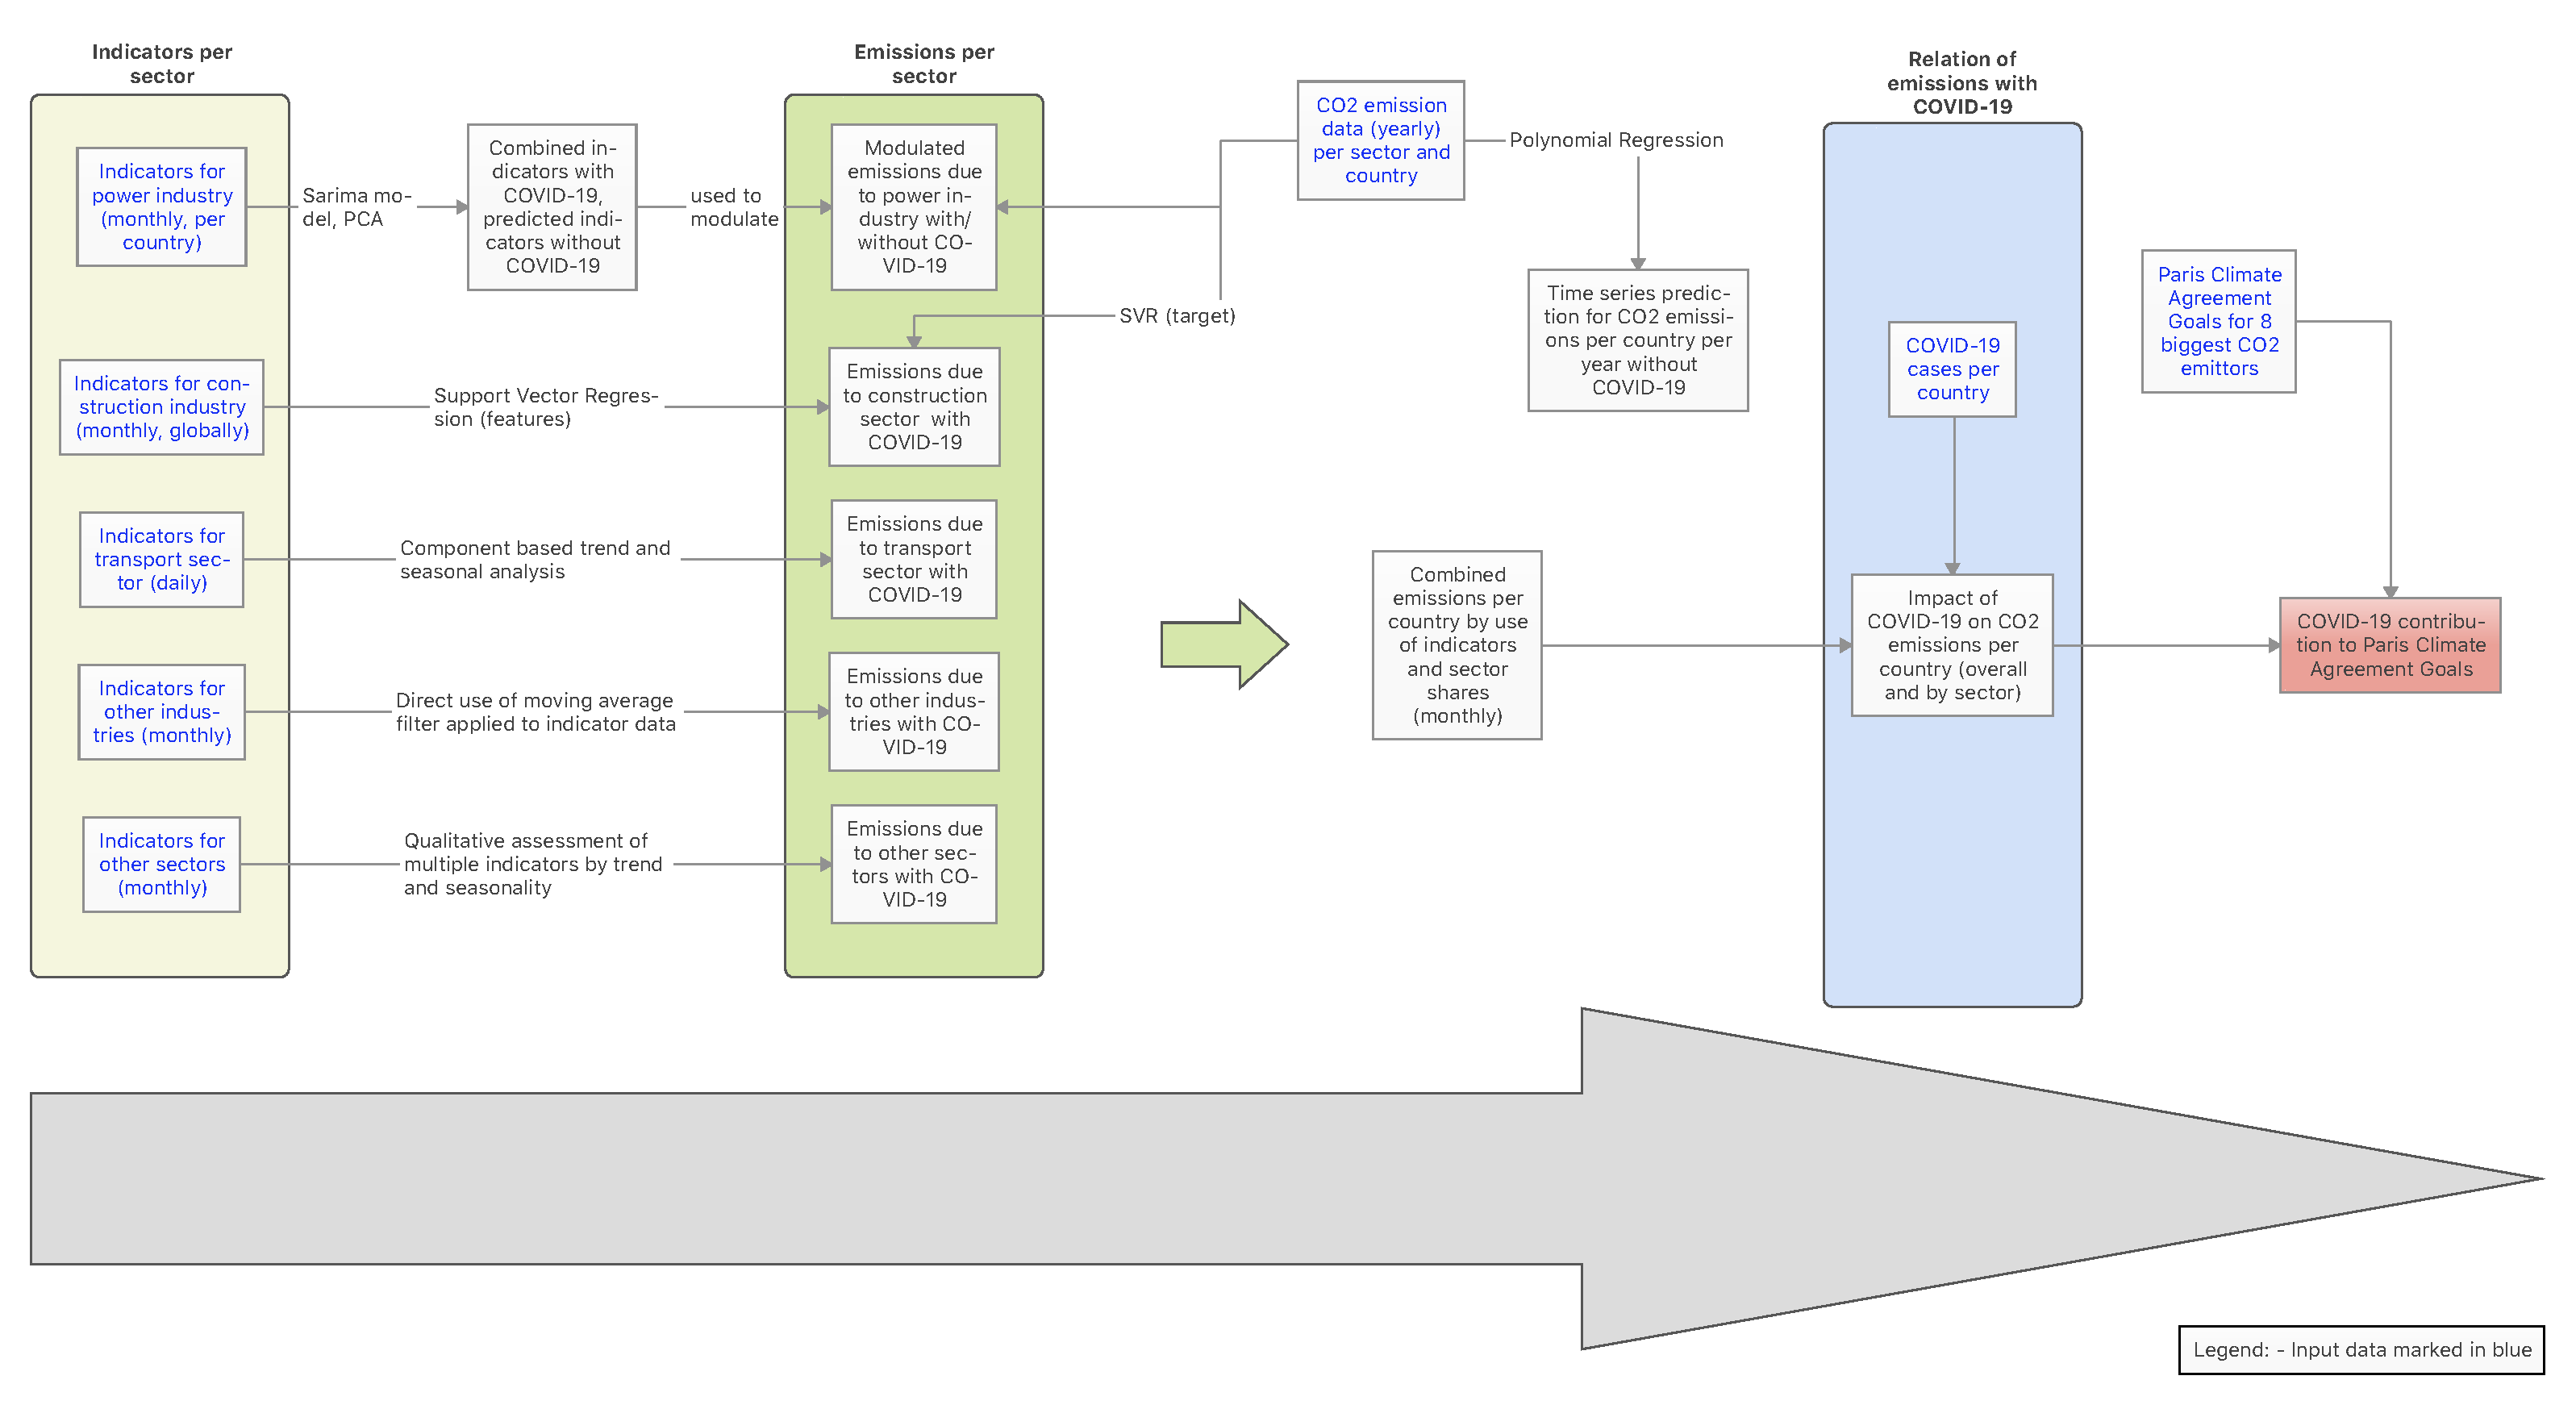
\includegraphics[width=1.45\linewidth, angle=90]{img/mock-up_frontend_pipeline_description.pdf}
	\caption{Depiction of the model pipeline. Input data is marked in blue.}
	\label{fig:model_pipeline}
\end{figure}




\section*{Model training}

%todo: Add Pipeline graphic from Max, should be full page, horizontally


\subsection*{Co2 prediction}

%todo: Explain CO2 prediction briefly
Our first idea was to get some datasets of indicators related to the corresponding sector with monthly data and up to date (at least up to May), that allowed us to predict how they would have behaved if the corona crisis would not have occurred. Then, after looking for the indicators, each sector prediction needed to be adapted according its indicators characteristics.


\subsection*{Sector summary}

%todo: For each sector: Indicator, ML Model, Evaluation, keep this short and concise
In the case of the power industry sector and the construction sector, the available data sets  allowed us to perform our original idea of predicting their normal behavior (without corona crisis) and compare it with the observed data. In the case of the transport sector and the other industries sector, it wasn't necessary to predict anything. For the other industries sector we only needed to adjust the seasonality of the indicators and normalize them. In the case of other sectors (mainly focused on agriculture) there was little data available and we were not able to compute a proper emission behavior. This is not optimal but since we can say that agriculture has seen little effect by the pandemic, we assume that there is no change.

\subsection*{Example: Power industry sector}

%todo: Select one example indicator (e.g. tranport) and explain how it was processed in more detail
We want to demonstrate how we computed the emission behavior for each sector by an example. We chose to do with the power industry sector.
For the power industry, we found four indicators: oil and power supply of the European countries and the brent and natural gas price. The first step was cleaning them so that they all started in 2008, normalizing them and separate them in different dictionaries. We separated them to differentiate between data before and after corona started; we set this date in December 2019. Then, we proceeded to search the indicator that was more correlated with the power industry emissions of each of the eight countries that produce the most \co emissions, assuming that they would behave in the same way after the start of the pandemic. With this, we trained a SARIMA model for each of the eight countries (seven countries and the European Union), where we predicted the behavior of the most correlated indicator.
In \autoref{fig:eu_prediction} we depict the prediction with and without the pandemic for the EU and summarize the resulting emission behavior for the power industry for all eight countries in \autoref{fig:power_ind_change_rate}.

Finally, we just compared the predicted versus the observed values of the indicators to generate a vector for each country with the fraction of \co emissions predicted between December and June.
Taking into account the lack of updated emissions data, we think that this is the best way to predict the drop in emissions if one is able to find good indicators.

\newpage

\begin{figure}[H]
	\centering
	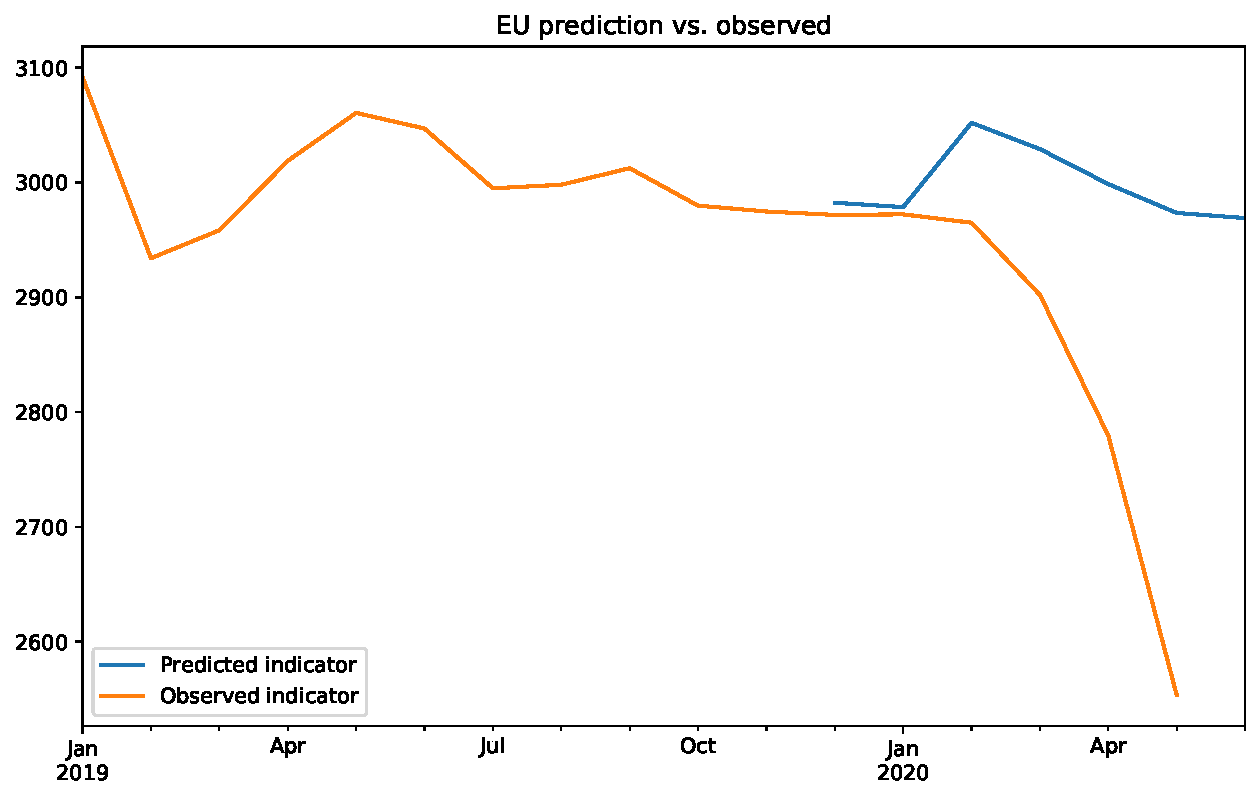
\includegraphics[width=0.85\textwidth]{img/EU_prediction.pdf}
	\caption{Predicted behaviour the best indicator for EU.}
	\label{fig:eu_prediction}
\end{figure}
%todo: Some text discussing it


%todo: Show resulting graph!!!
\begin{figure}[H]
	\centering
	\includegraphics[width=0.9\textwidth]{img/Power_industry_rate.pdf}
	\caption{Predicted behavior of the power industry for all countries considered. For most countries we see lowered emissions. For the EU we observe almost steady \co emissions.}
	\label{fig:power_ind_change_rate}
\end{figure}


\section*{Evaluation}

%todo: How valid are the results?
As previously discussed, it was crucial to have good indicators, this means having indicators highly correlated with the emissions of the corresponding sector.

% Task: Are the models good?
In the case of the power industry sector, we achieved high correlations for most of the countries. Probably with specific indicators for each country, correlations would have been better. This is complicated especially in the case of China, which has a very strict policy on sensitive data.
For the construction sector, the indicators used have different factors that affect them other than emissions. Therefore, the achieved correlations were not as good.
For the mobility sector, the dataset found already provided us the change in mobility which is, presumably the change in emissions. For the other industries sector, we had a similar case.
The emission behavior of the other sectors purely relies on our assumption that it will behave exactly as without the pandemic. This inflicts high uncertainties of course. For most countries, other sectors only contribute 10\% or less to the country's emission however. Therefore, it should not influence our final result as much.


\section{Results and Discussion}

This section contains our main results and the discussion. First, we present our \co prediction, which is the output from our trained sector models. Afterwards, we dig deeper into our data, and reveal, which sectors were de- or increasing the most. The second part is dedicated to the analysis of the COVID-19 impact, where we briefly analyze the developments so far, and correlate different metrics in a time series fashion and a simpler integrated correlation plot. The third part relates those correlations with the goals of the paris climate agreement. Finally, we conclude the section with a thorough discussion of the validity of our data and an answer to the research question.

\subsection*{\co emission drop in all countries}

We start with presenting the main result of our sector resolved \co prediction approach. In Figure \ref{fig:expected_change_rate}, the predicted change rates per month and country are illustrated.

\begin{figure}[H]
	\centering
	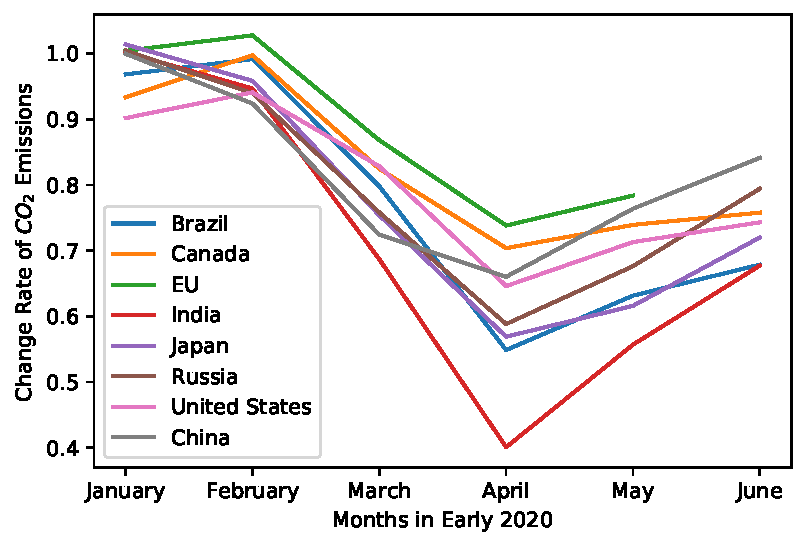
\includegraphics[width=0.7\textwidth]{img/change_rate.pdf}
	\caption{Overall expected change rate.}
	\label{fig:expected_change_rate}
\end{figure}

Here we can observe that the emissions were more or less the same during January and February, just before the beginning of the corona crisis. Then, from March on, when countries followed Chinas lock down approach with their own policies, we can see a clear drop in emissions, resulting in a \co emission performance between 0.8 and 0.4. From May on, the lock-down phase was abolished in many countries. This explains that the emissions start climbing again to a pre-COVID-19 regime.

In summary, the relative emission drop was most prominent in India (down to 40\%), whereas the EU, Canada, USA and China showed a more robust response of minimum emission values around 70\%.

In fact, COVID-19 impacted India's economy probably more severely then others. According to an article published by Maurice Kugler and Shakti Sinha in July 2020, 400 million people risk falling into poverty due to COVID-19 \cite{Kugler}, which is not only a significantly larger fraction of the population than in any other country, but also a more substantial threat than temporal unemployment.

\subsection*{Sector trends: Power industry as the leading sector}%todo: Pie charts

But what led to the decrease of emissions in the first place? We try to approach this question, by analyzing the individual performance of single sectors in each country. For the different plots in Figures \ref{fig:bar_plots} and \ref{fig:bar_plots2}, the performance vectors where averaged over the period of the year 2020 so far.

\begin{figure}[H]
	\centering
	\subfloat[Brazil]{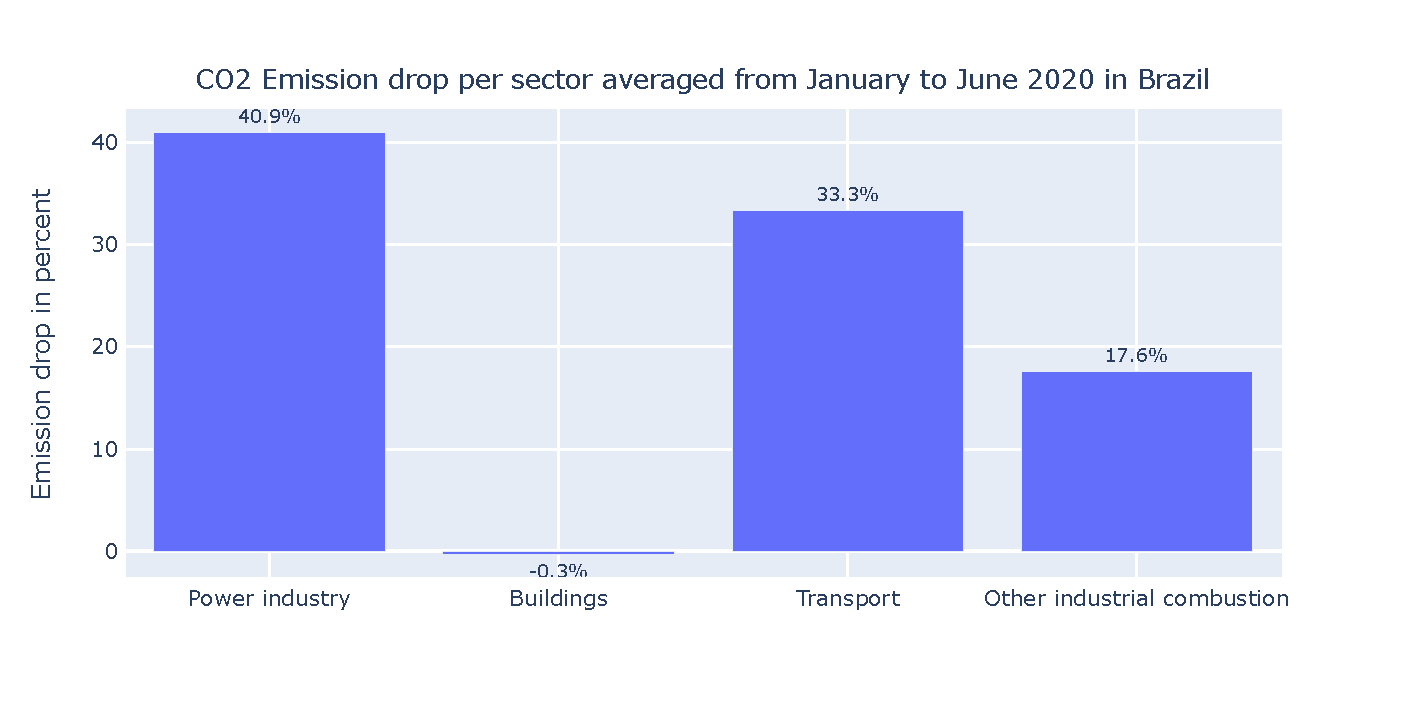
\includegraphics[width=0.45\linewidth]{../sector_overview/bar_plot_Brazil}}
	\subfloat[Brazil]{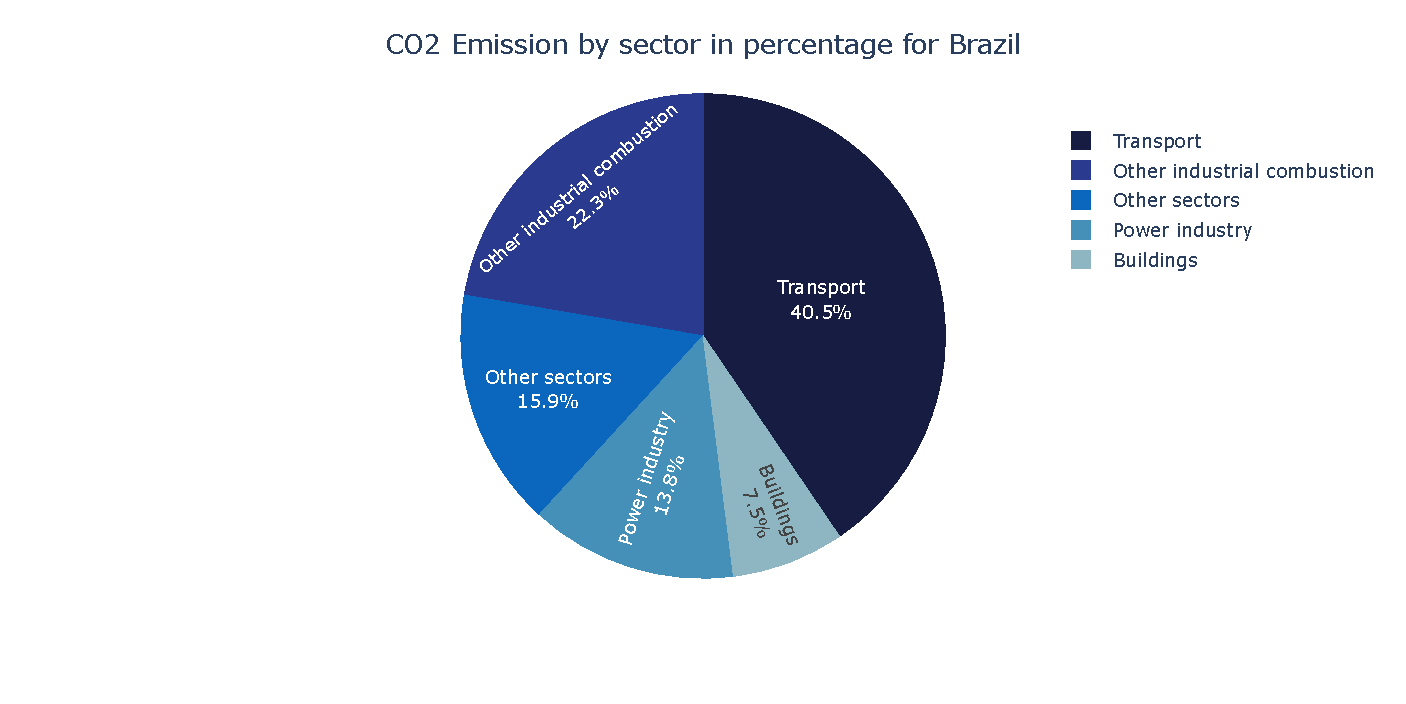
\includegraphics[width=0.45\linewidth]{../sector_overview/pie_plot_Brazil}}\\
	\subfloat[Canada]{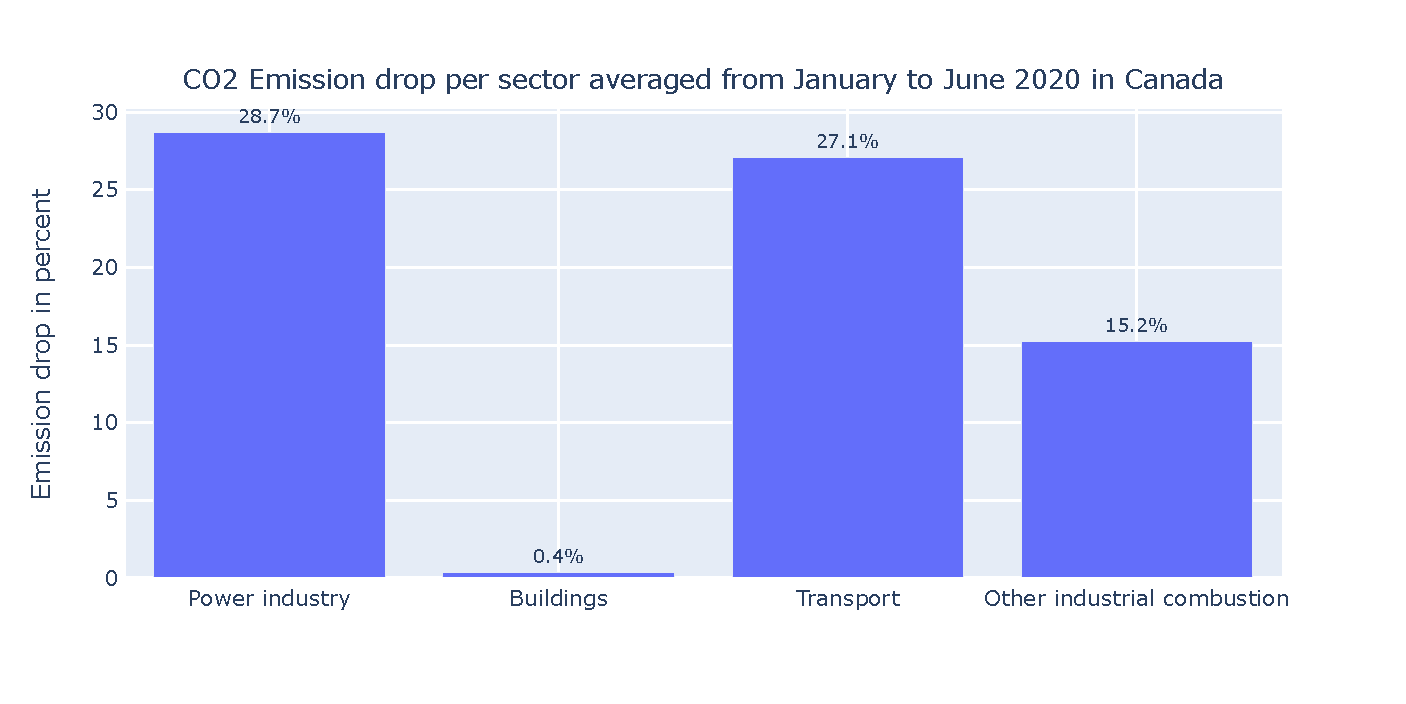
\includegraphics[width=0.45\linewidth]{../sector_overview/bar_plot_Canada}}
	\subfloat[Canada]{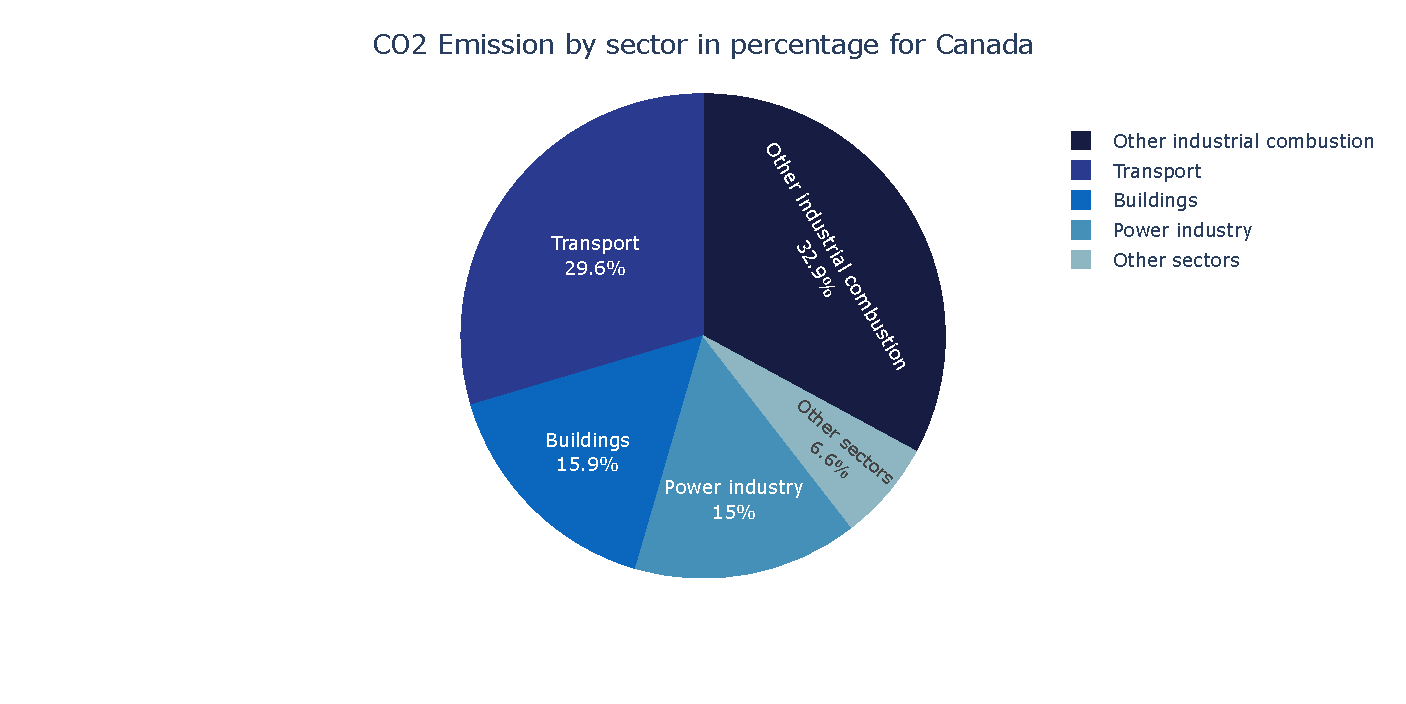
\includegraphics[width=0.45\linewidth]{../sector_overview/pie_plot_Canada}}\\
	\subfloat[China]{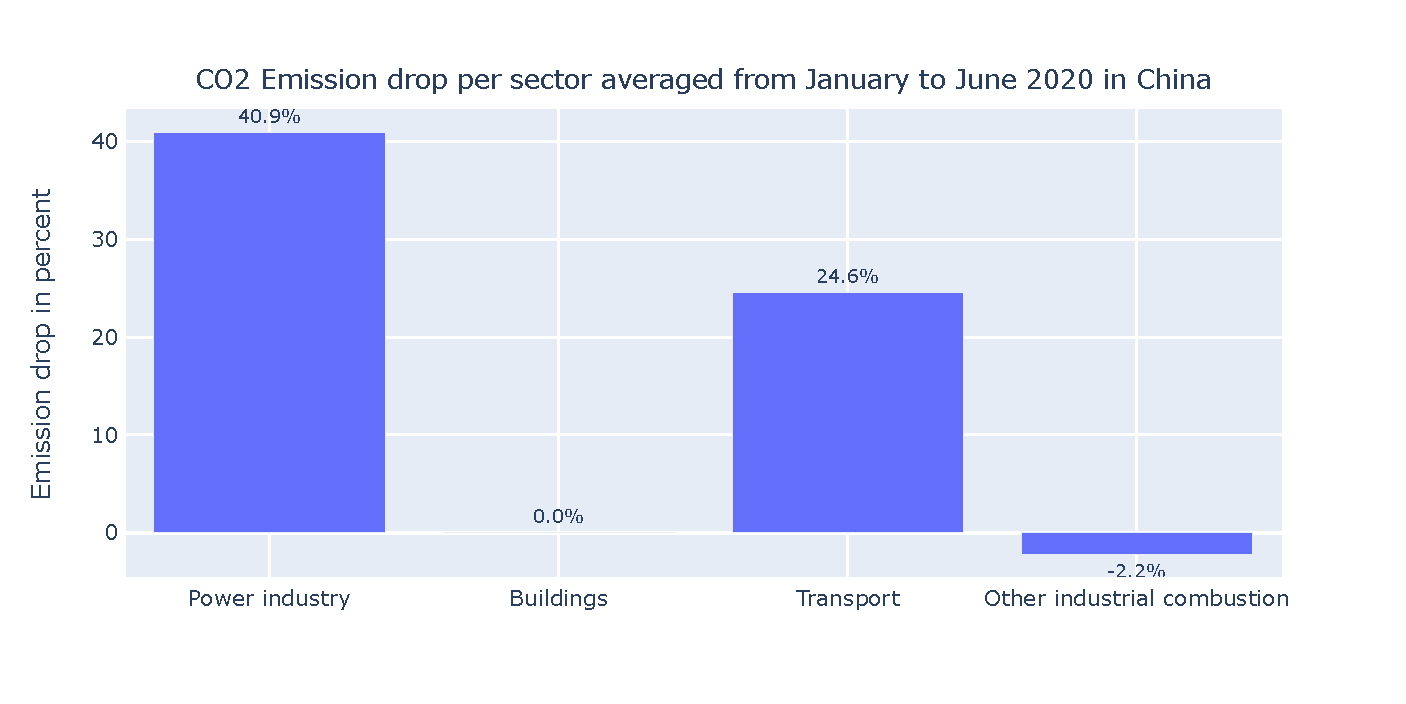
\includegraphics[width=0.45\linewidth]{../sector_overview/bar_plot_China}}
	\subfloat[China]{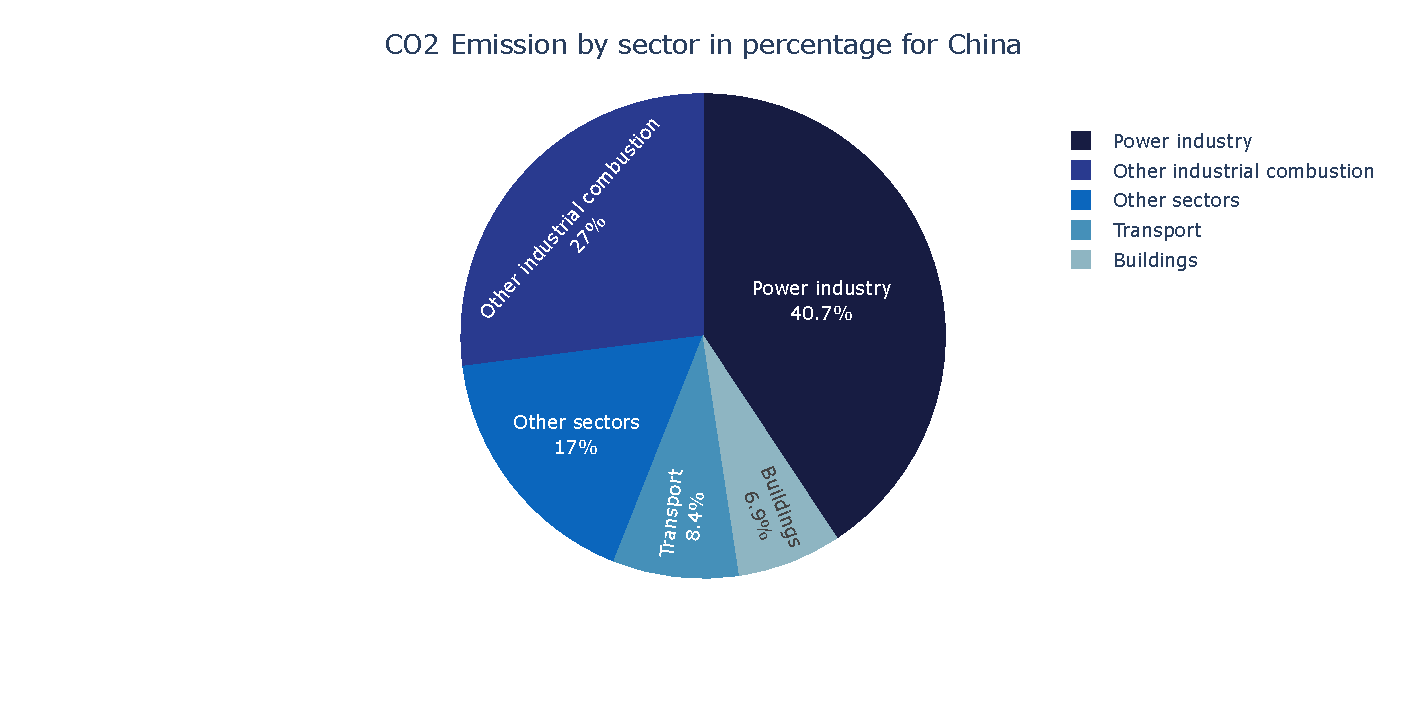
\includegraphics[width=0.45\linewidth]{../sector_overview/pie_plot_China}}\\
	\subfloat[EU]{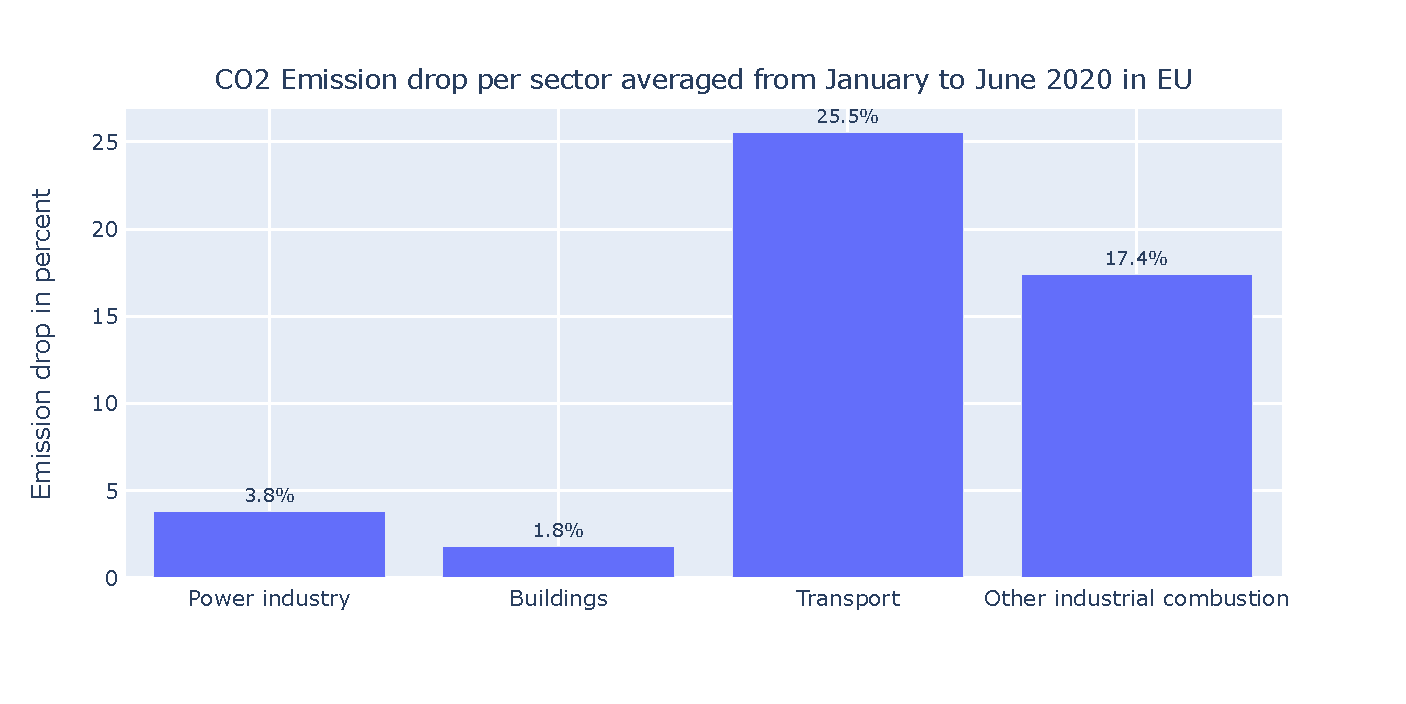
\includegraphics[width=0.45\linewidth]{../sector_overview/bar_plot_EU}}
	\subfloat[EU]{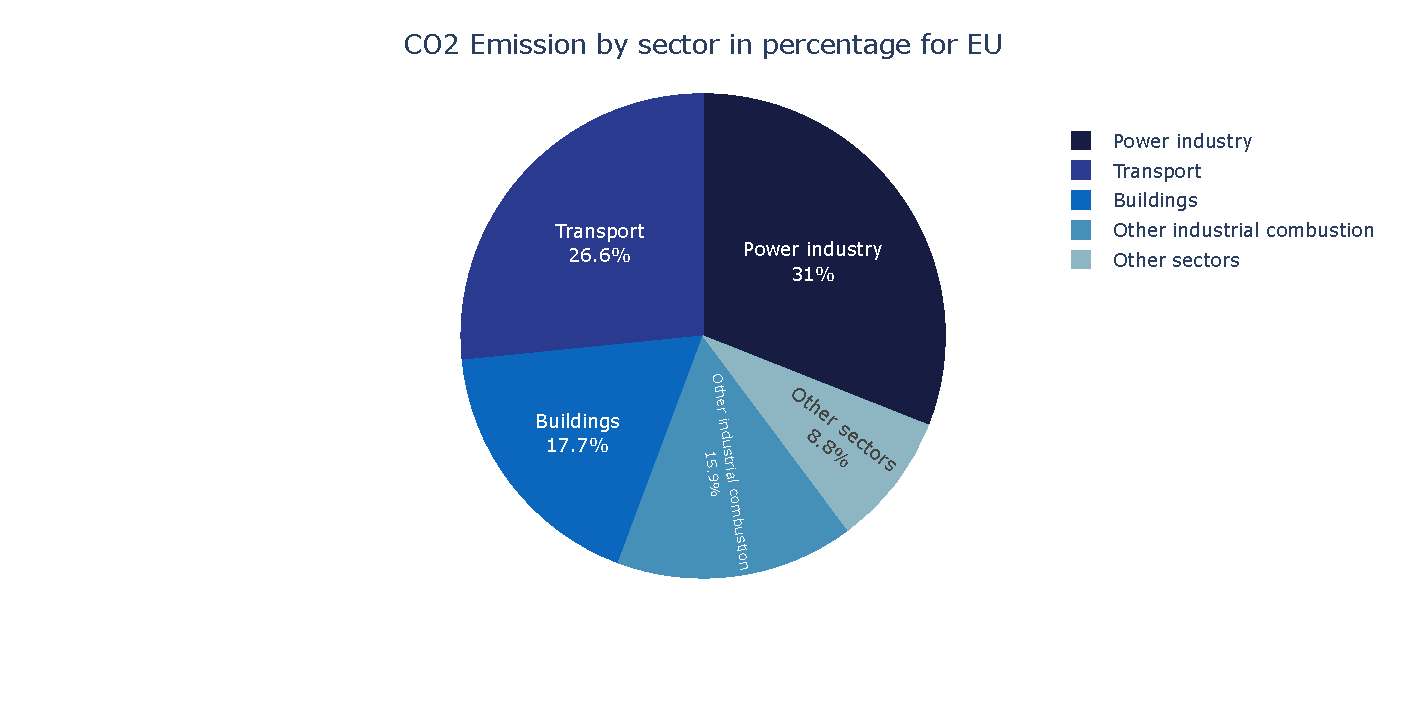
\includegraphics[width=0.45\linewidth]{../sector_overview/pie_plot_EU}}\\
	\caption{Averaged emission drop from January to June 2020 per country.}
	\label{fig:bar_plots}
\end{figure}

\begin{figure}[H]
	\centering
	\subfloat[India]{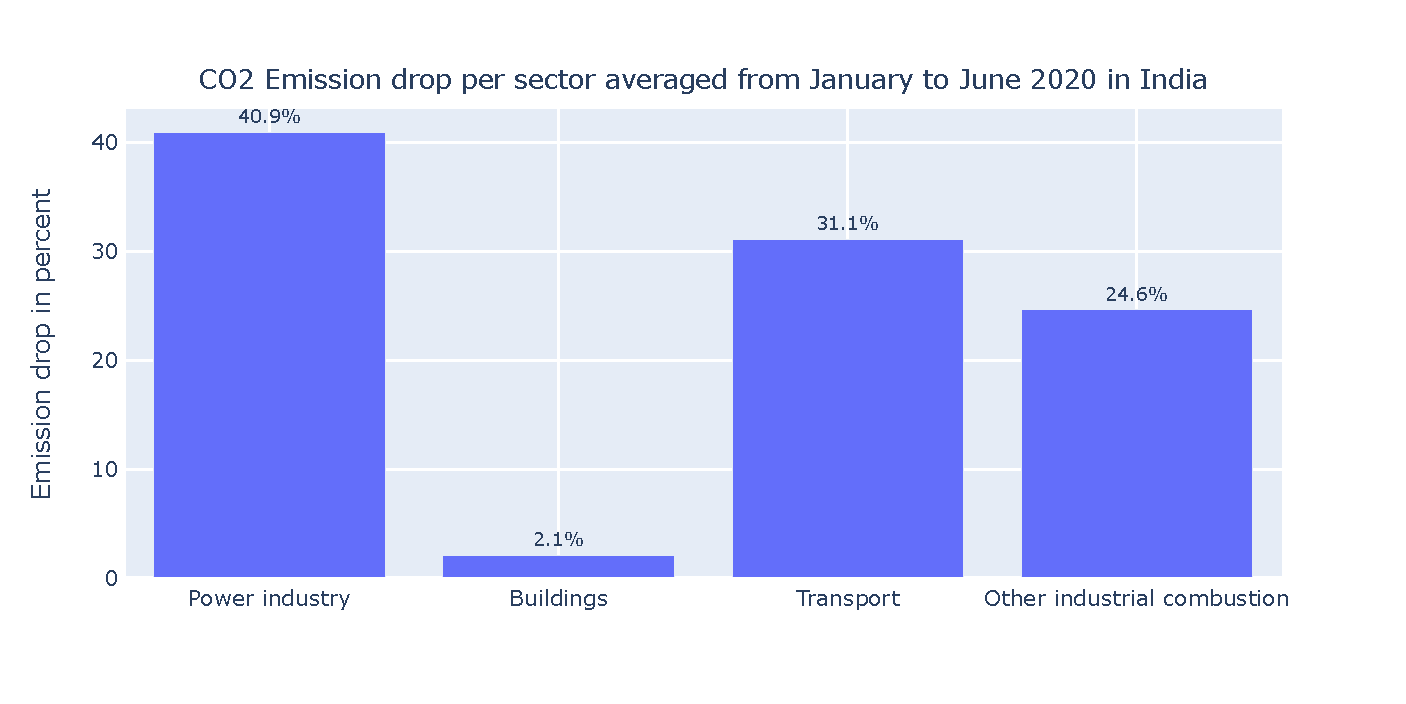
\includegraphics[width=0.45\linewidth]{../sector_overview/bar_plot_India}}
	\subfloat[India]{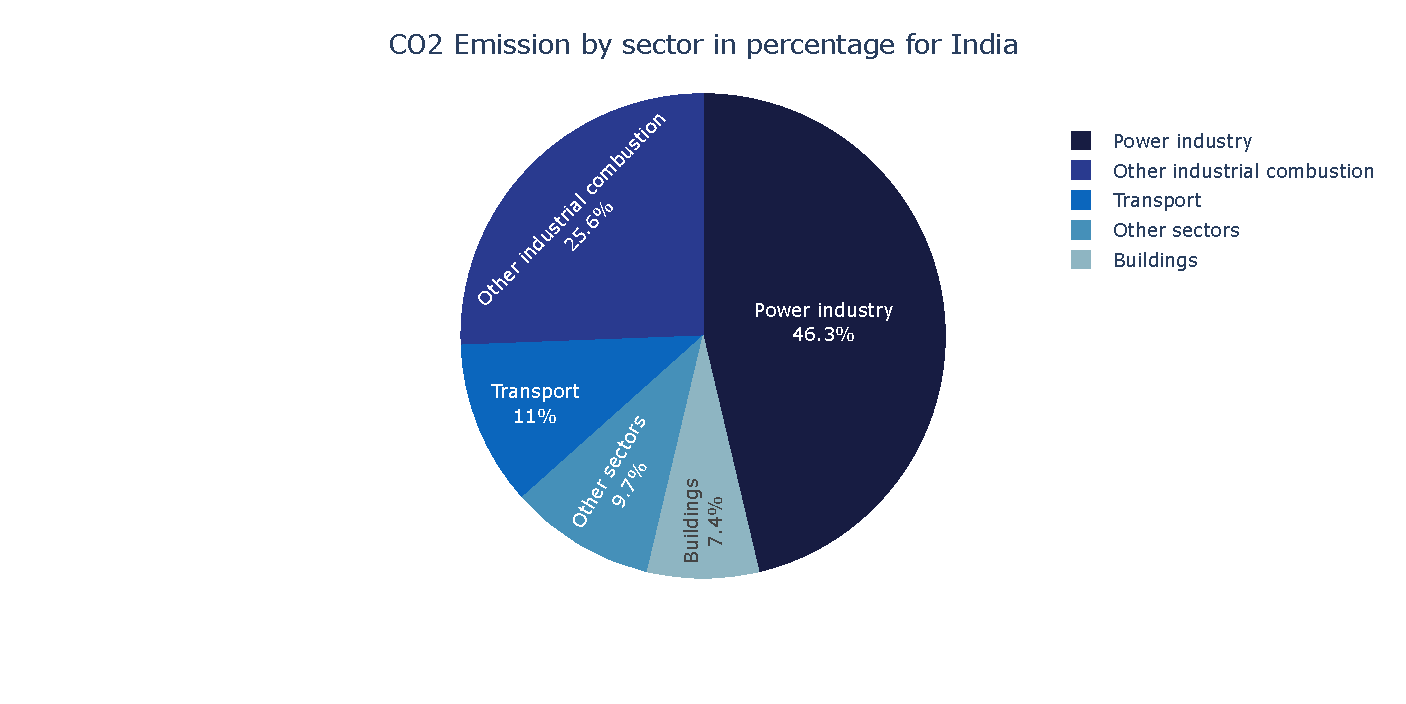
\includegraphics[width=0.45\linewidth]{../sector_overview/pie_plot_India}}\\
	\subfloat[Japan]{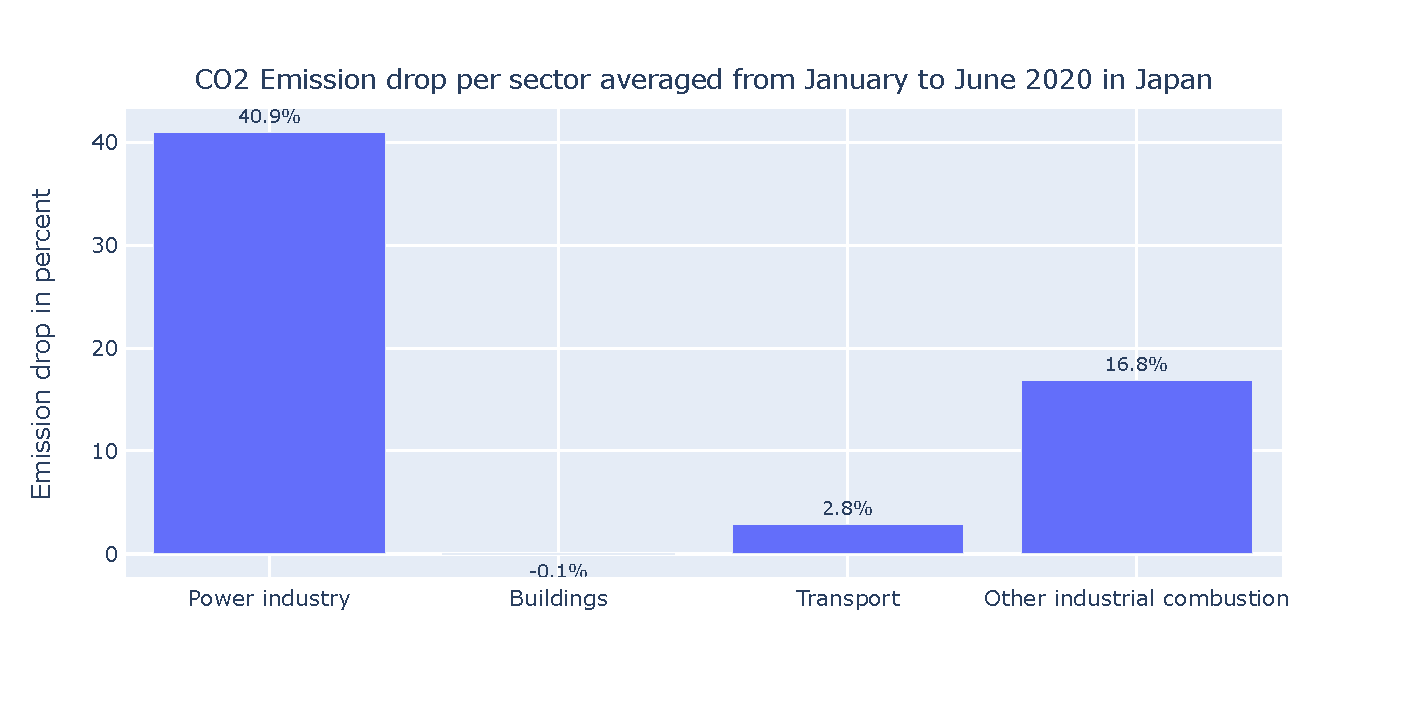
\includegraphics[width=0.45\linewidth]{../sector_overview/bar_plot_Japan}}
	\subfloat[Japan]{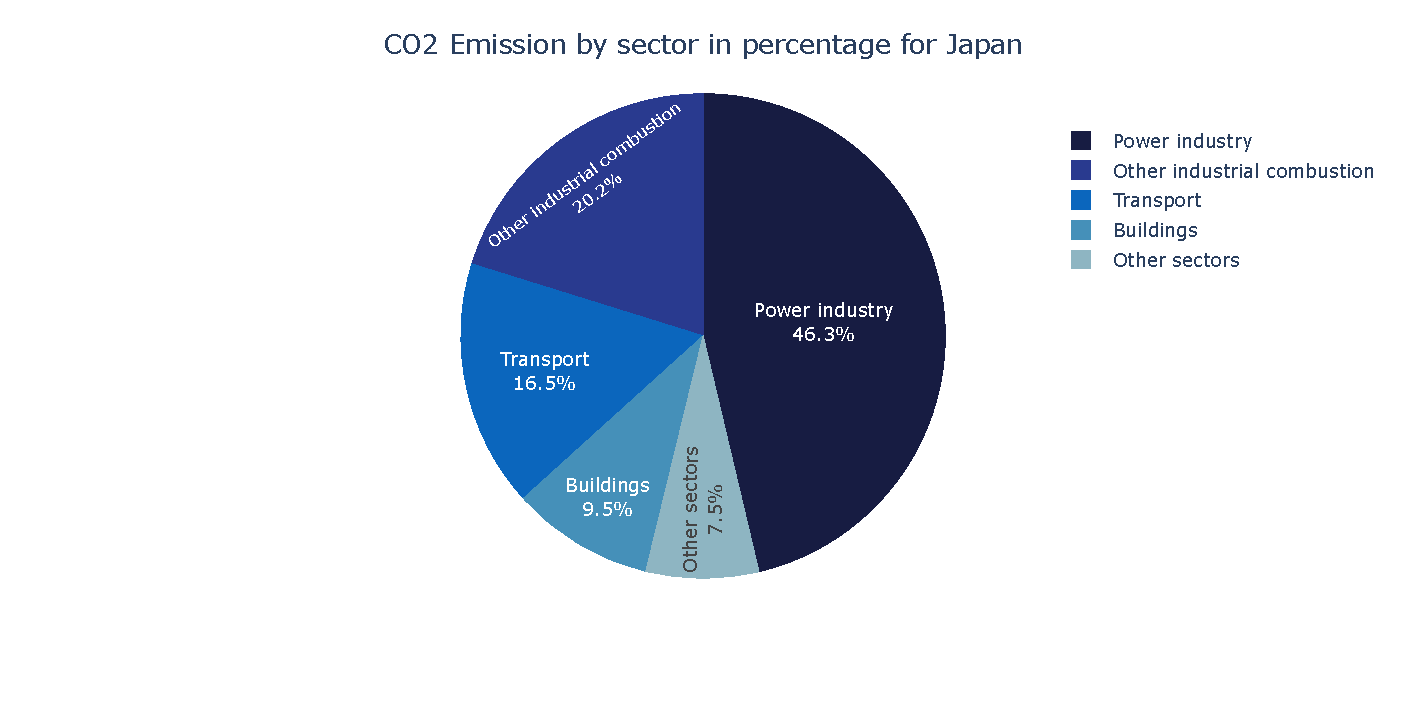
\includegraphics[width=0.45\linewidth]{../sector_overview/pie_plot_Japan}}\\
	\subfloat[Russia]{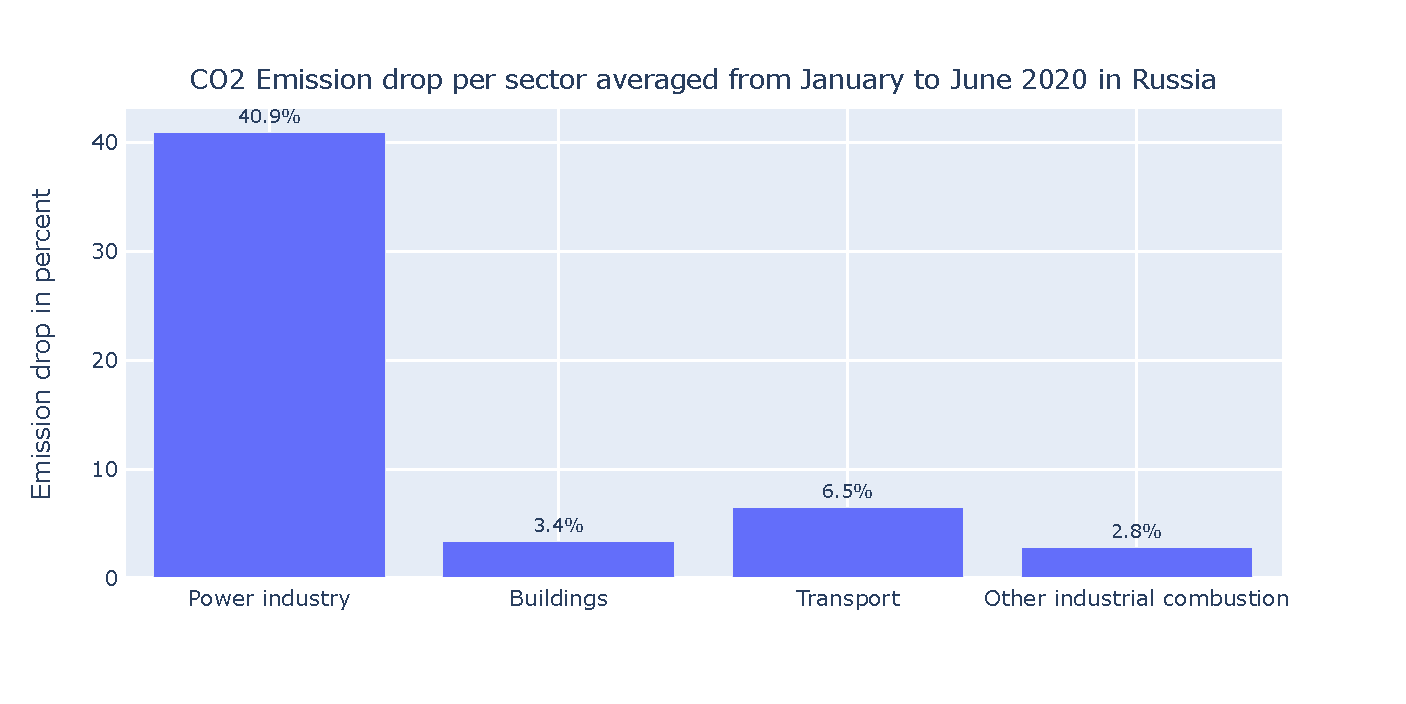
\includegraphics[width=0.45\linewidth]{../sector_overview/bar_plot_Russia}}
	\subfloat[Russia]{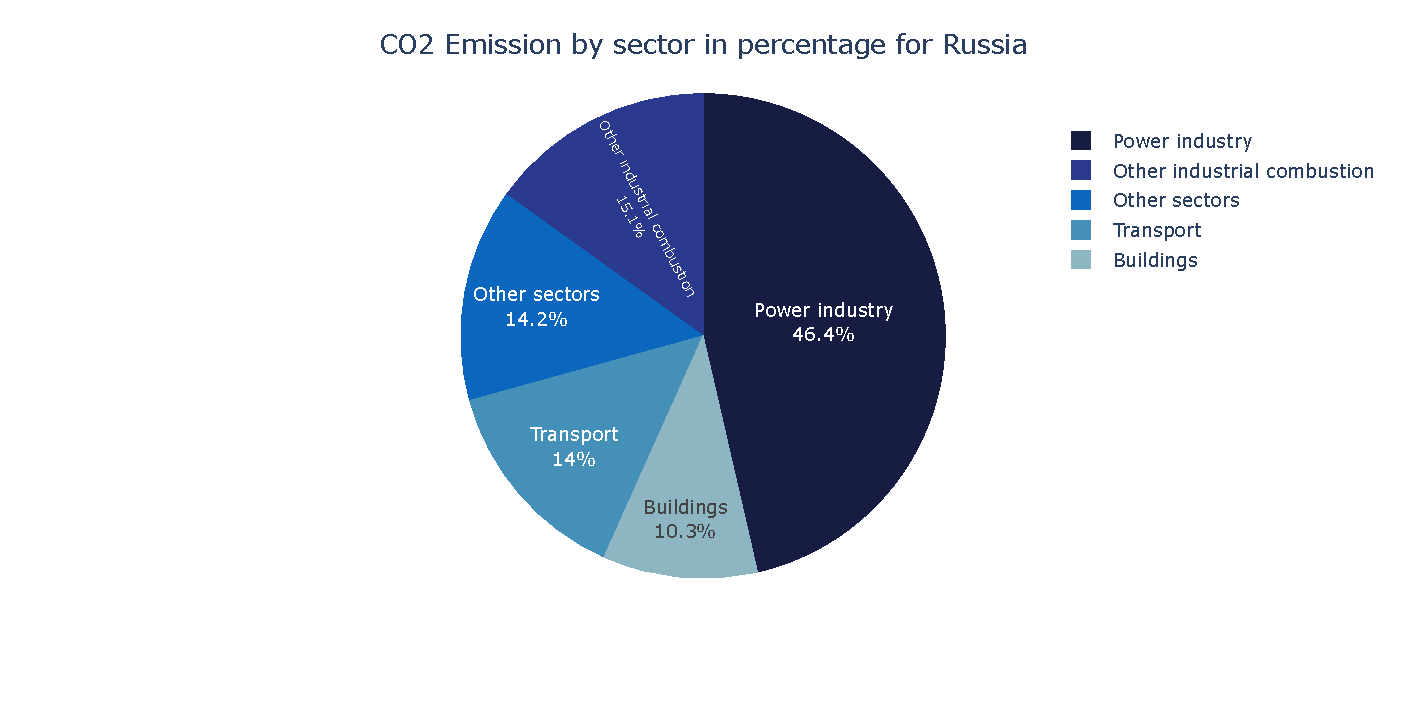
\includegraphics[width=0.45\linewidth]{../sector_overview/pie_plot_Russia}}\\
	\subfloat[United States]{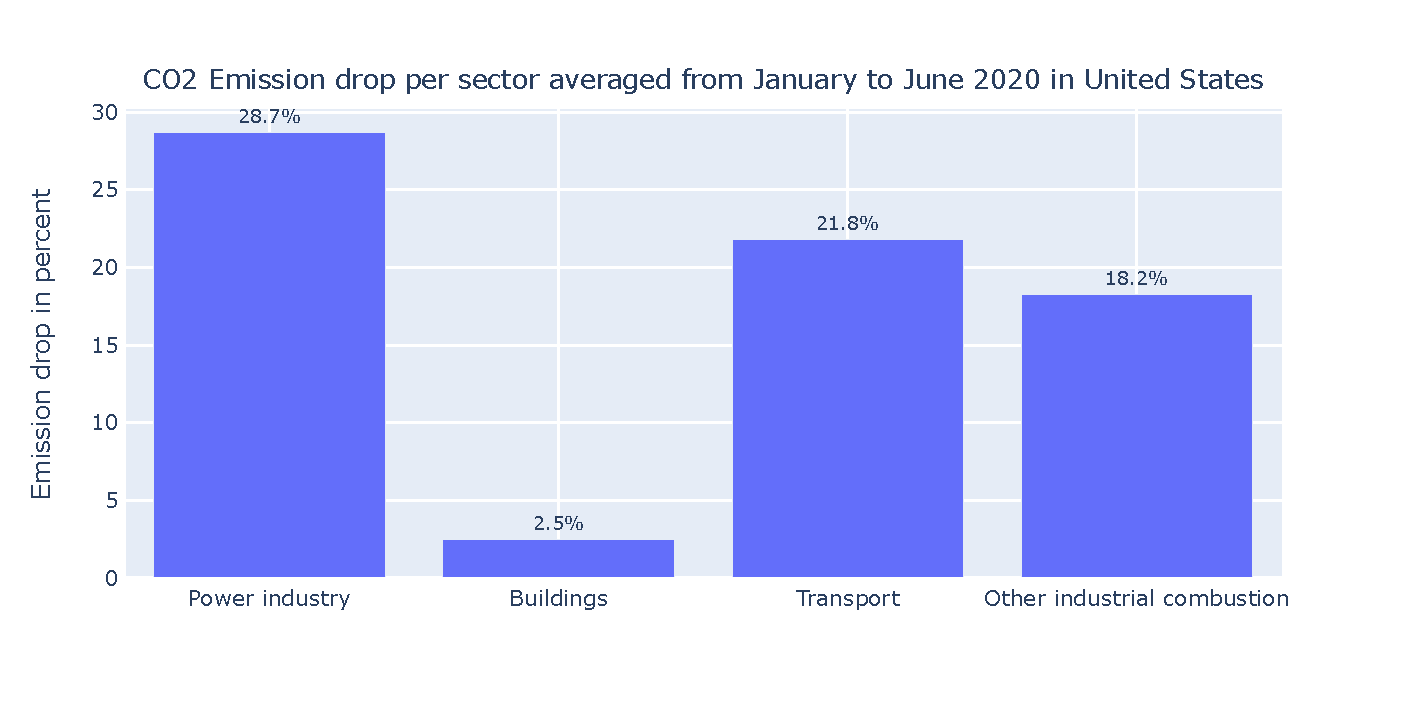
\includegraphics[width=0.45\linewidth]{../sector_overview/bar_plot_United_States}}
	\subfloat[United States]{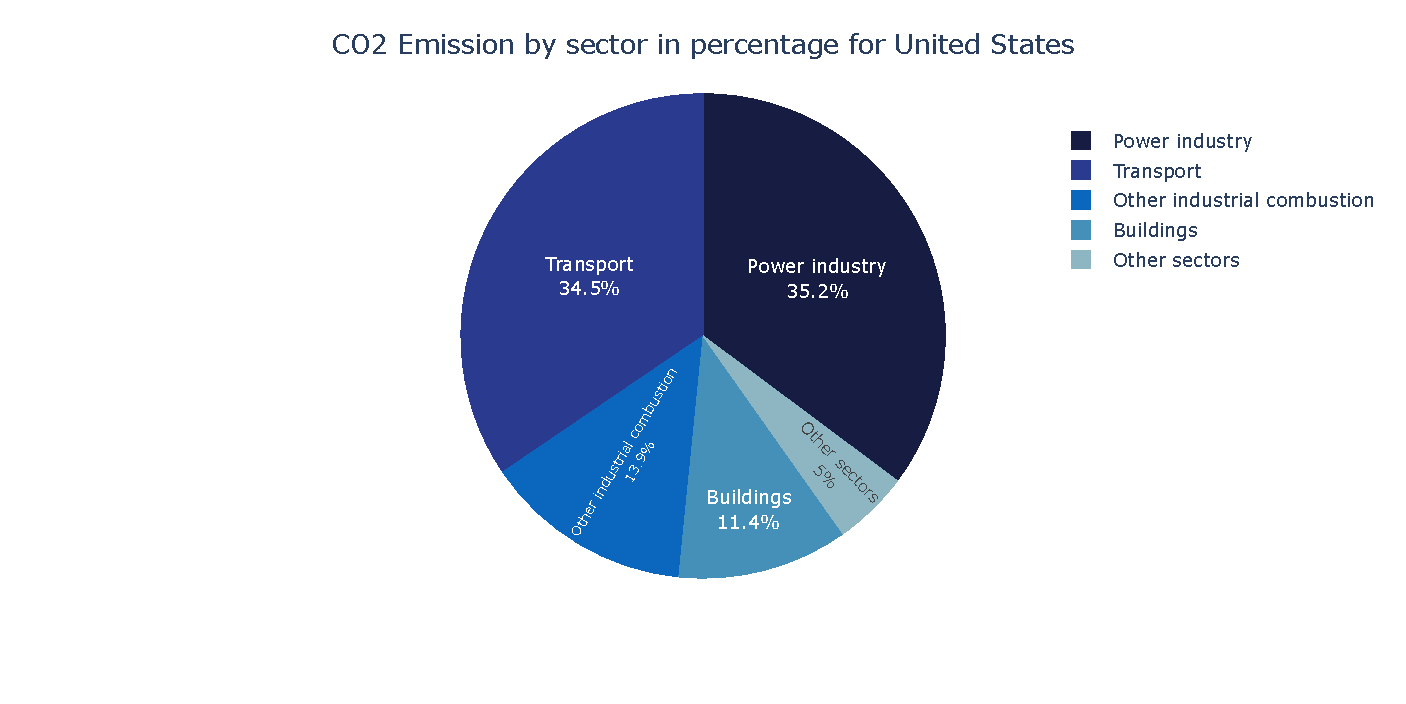
\includegraphics[width=0.45\linewidth]{../sector_overview/pie_plot_United_States}}
	\caption{Averaged emission drop from January to June 2020 per country.}
	\label{fig:bar_plots2}
\end{figure}

Even without inspection, one can easily identify the consistently most impacted sector to be the power industry of $20-40\%$. This sector includes fuel generation in general, which was in much less demand since February one could argue. The only region showing no significant decrease is the EU. This can be explained by the low fuel production in general, leading to a more stable profile.

The second sector of interest is the building sector. Here, remarkably low changes of $<5\%$ can be noted. In fact, one could conclude that the construction industry remained active during the pandemic. Also in Munich, we experienced a lot of construction activity for public projects like road improvements.

The third sector is the transport sector. We can note big decreases for Brazil, Canada, China, EU and the USA. 
Naturally, the travel activity in general is indicated by the performance of this sector. An explanation for Japan's low change in transport can be found, when we consider that Japan was among the last countries to start travel bans.
It remains unclear why Russia shows also less fluctuations.

The sector for other industrial combustions is connected to the production of goods. While China and Russia remained unaffected, all other countries in this analysis had a decent emission drop in this sector. China did a good job in confining the virus early, leading to less severe restrictions for the workforce in general. Russia's economy is more centered around fuel generation.

In conclusion, the biggest impact was the decrease of fuel production and transportation in general.



\subsection*{Largest COVID-19 impact for American and European continents}
\begin{figure}[H]
	\centering
	\subfloat[Cumulated cases per 100k inhabitants]{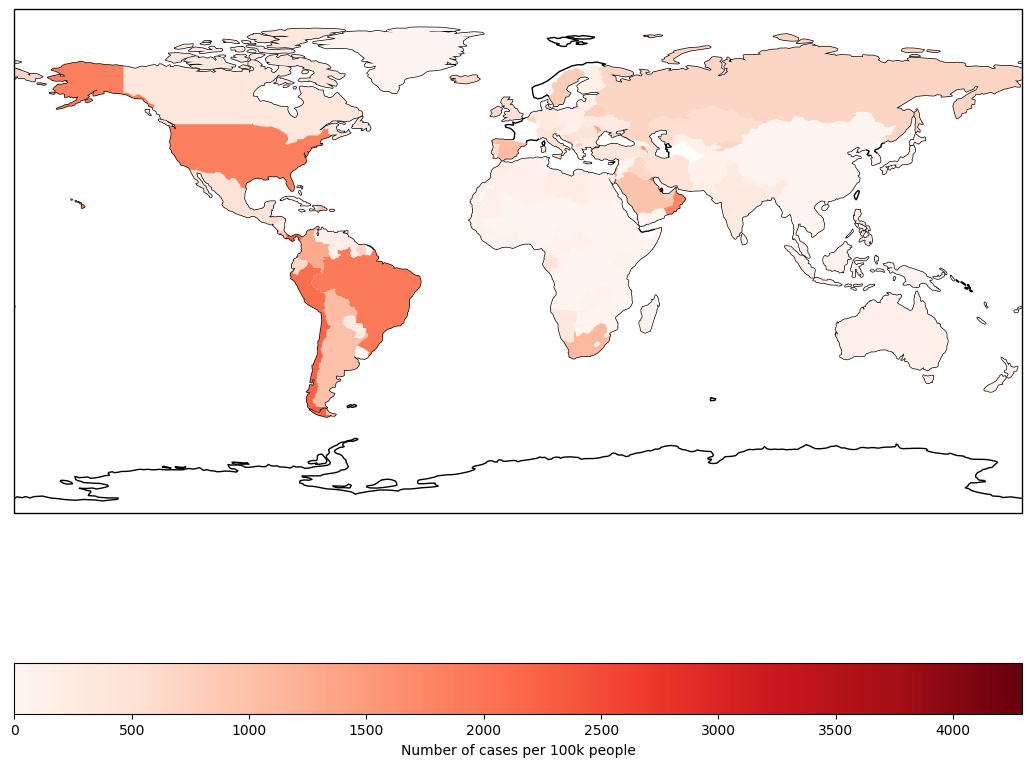
\includegraphics[width=0.5\textwidth]{../covid/case_rate.png}}
	\subfloat[Cumulated deaths per 100k inhabitants]{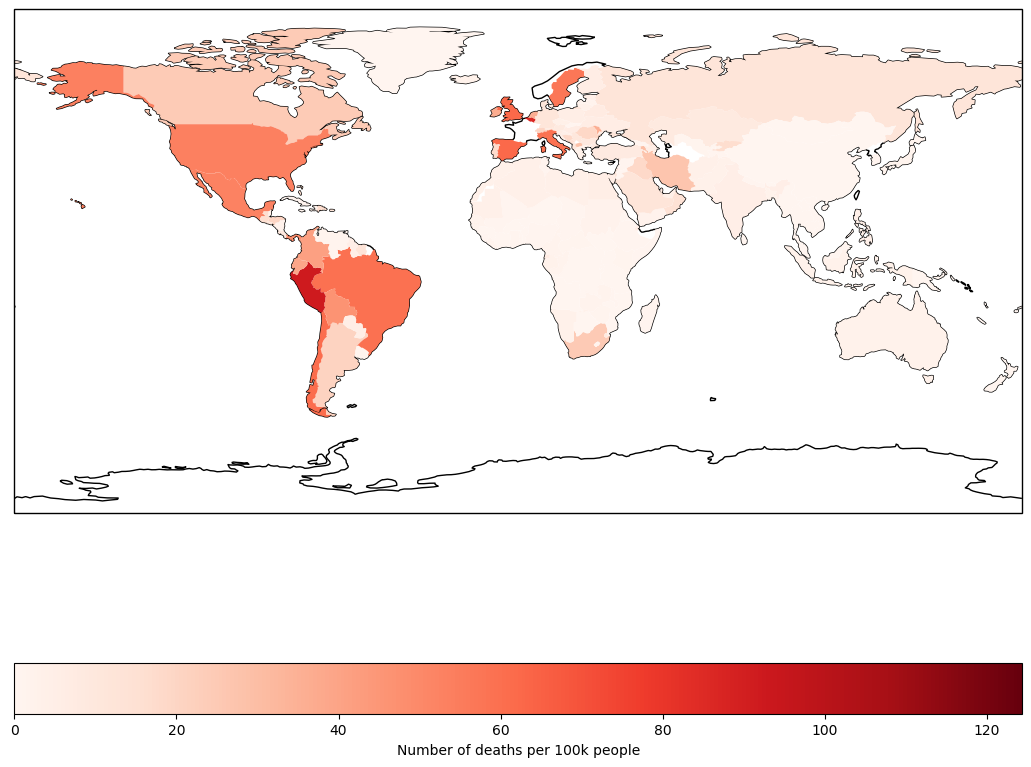
\includegraphics[width=0.5\textwidth]{../covid/death_rate.png}}
	\caption{COVID-19 impact visualization.}
	\label{fig:covid_cases}
\end{figure}% rate means per 100.000 inhabitants

As this report focuses on the impact of COVID-19 in \co emissions, we generated different maps to see the impact of COVID-19 all around the world. In combination with a dataset for the population in each country, we could normalize the cumulated deaths and cases by the population number to normalize the size of one country.

In Figure \ref{fig:covid_cases}, the case and death numbers per country are shown. Here, we can observe that the countries affected the most are the United States, Brazil and parts of the EU, which also are three of the eight countries that produce the most \co emissions. This reassures our choice of picking the eight biggest industries of the world, as we can hope for finding correlations.

\subsection*{No evidence with time series COVID-19 correlation}
In order to find a relation between the \co emissions and the COVID-19 data one can use the Pearson or the Spearman correlation between the predicted vectors from the different sectors and the death, active, and confirmed cases.

The correlation coefficient according to Pearson is sensitive to outliers. Therefore, we used the spearman method to identify the correlation coefficient.

\begin{figure}[h!]
	\centering
	\subfloat[COVID-19 data compared to the predicted overall vector for Japan]{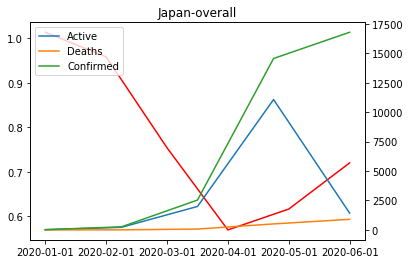
\includegraphics[width=0.5\linewidth]{ziedPNGS/japanOverall}}
	\subfloat[COVID-19 data compared to the predicted overall vector for EU]{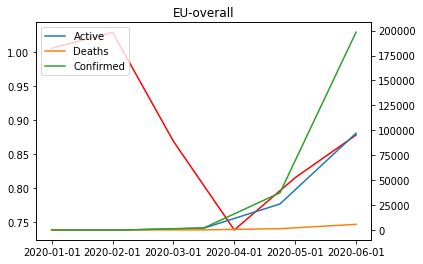
\includegraphics[width=0.5\linewidth]{ziedPNGS/euOverall}}
	\caption{Comparison between the predicted vectors and Covid-19 data.}
	\label{fig:Covid-predictedVectors}
\end{figure}

\begin{center}
\begin{table}[h!]
	\centering
	\begin{tabular}{llllll}
		\hline
		 Countries&Overall&buildings&mobility&power industry&other industries\\
		\hline
		\hline
		 Canada   & -0.6 & -0.6& -0.6& -0.999& -0.999\\
  		 China &  -0.199 & 0.7& -0.899& 0.099& -0.399\\
 		 Japan & -0.899 & 0.6& -0.999& -0.799& -0.7\\
 		 Russia &0.099 & -0.899& -0.099& -0.099& -0.799\\
  		 Brazil & -0.6 & 0.3& -0.6& -0.3& -0.7\\
		 India & -0.499& -0.899& -0.499& -0.099& -0.499\\
 		 United States & -0.714 & -0.028& -0.714& -0.428& -0.942\\
		 EU &-0.542 & -0.828& -0.542& -0.714& -0.714\\
		\hline &\\
	\end{tabular}
	\caption{Spearman correlation.}% linear
	\label{tab:spearman}	
\end{table}	
\end{center}

Even if the results show a negative correlation for some sectors activities and the CO2 emissions, only Japan's overall emissions seems to be affected by the increase of the COVID-19 cases.

A light tendency can be observed for the United States and the EU. By closer inspection in Figure \ref{fig:Covid-predictedVectors}, no strong relationship could be determined.

\subsection*{Nonlinear cumulated emission-COVID-19 correlation}

Therefore, we tried to correlate the integrated COVID-19 impact and the integrated emission drop. These correlations can be observed in Figure \ref{fig:emission_drop_over_normalized_deaths}. 

\begin{figure}[h!]
	\centering
	\subfloat[cases]{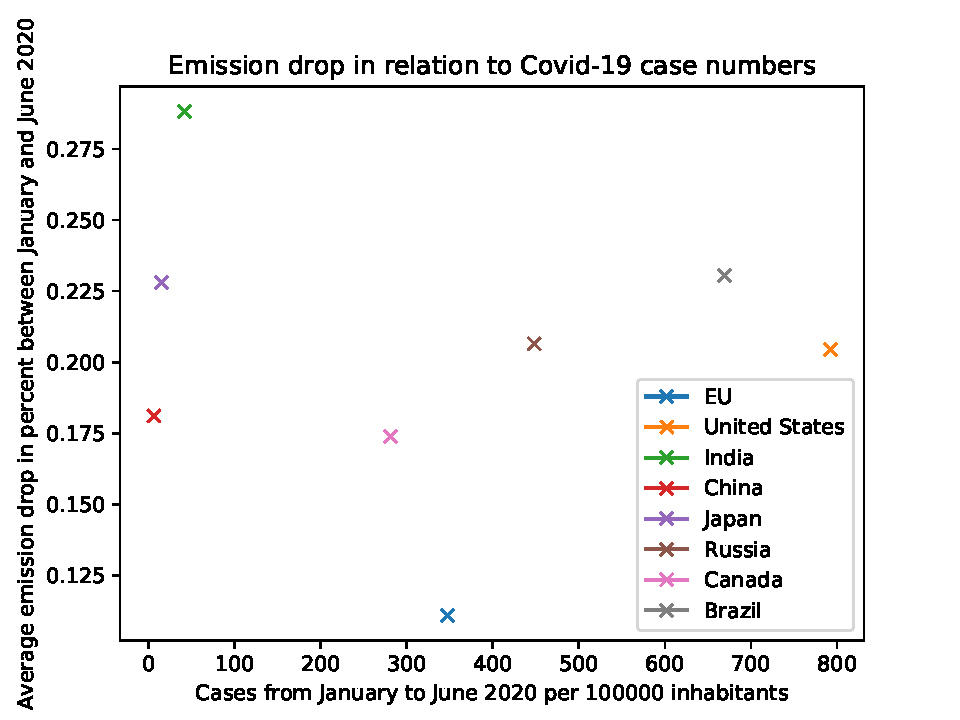
\includegraphics[width=0.5\linewidth]{../final_results/emission_drop_over_normalized_cases}}
	\subfloat[deaths]{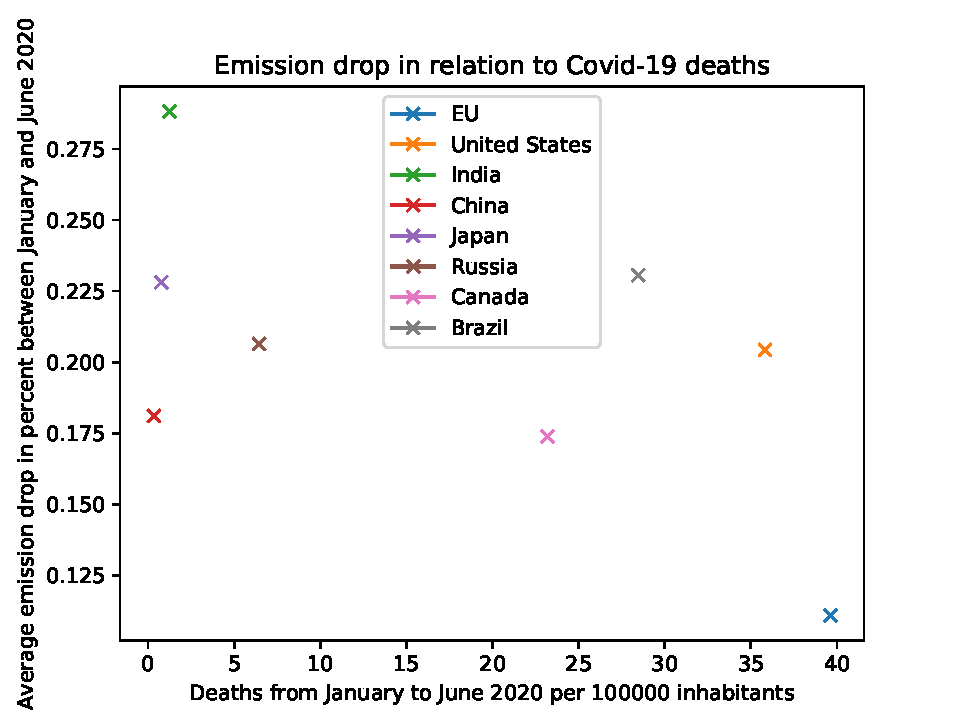
\includegraphics[width=0.5\linewidth]{../final_results/emission_drop_over_normalized_deaths}}
	\caption{Emission drop relation to COVID-19 case/death numbers.}
	\label{fig:emission_drop_over_normalized_deaths}
\end{figure}

In contrary to what we hoped, no linear trend could be extracted. Therefore, each country has to be evaluated independently. Two reasons could give rise to the noisiness: Either, there is no per country correlation, as the economies of different countries work differently and the complex net of globalization is not trivial to analyze, or our approach has significant weaknesses. Possibly, a combination of both makes this result plausible.

\subsection*{Relation to paris climate goals}

Even though no linear trend between COVID-19 cases and the \co emission drop could be seen in our analysis, one can still note the significant decrease in emissions during the corona crisis. In \autoref{fig:goals_lines}, the Paris climate goals of the biggest eight contributors are plotted in two ways. Subfigure (a) shows the reference year and the drop at the goal year, while Subfigure (b) normalizes the reference years to get a sense of the ambitiousness of each country.

\begin{figure}[H]
	\centering
	\subfloat[Compared to Referenced Year]{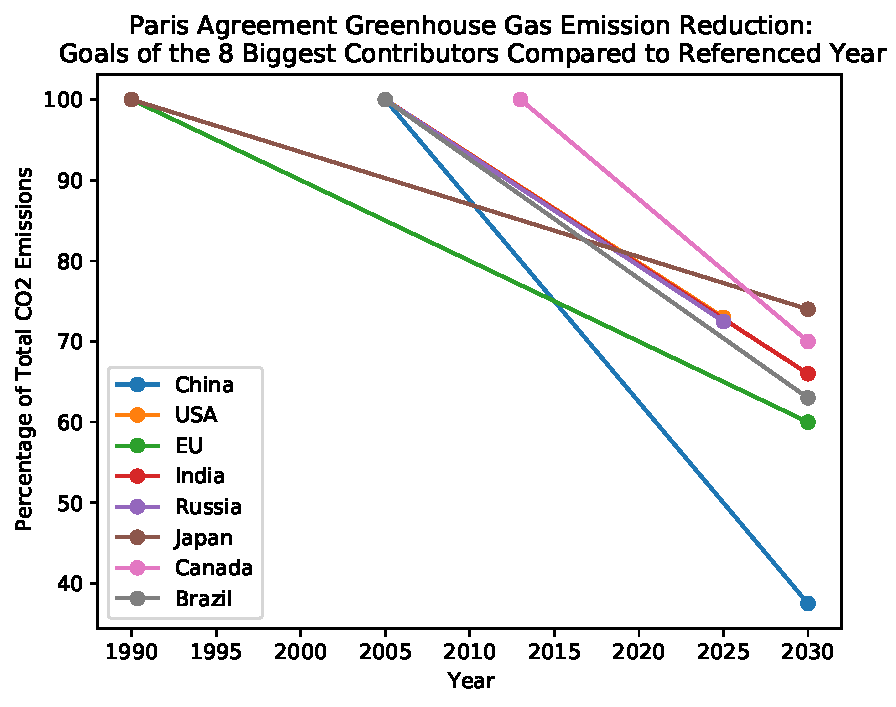
\includegraphics[width=0.5\textwidth]{img/co2goals_lines.pdf}}
	\subfloat[Compared to the 1.5°C Goal]{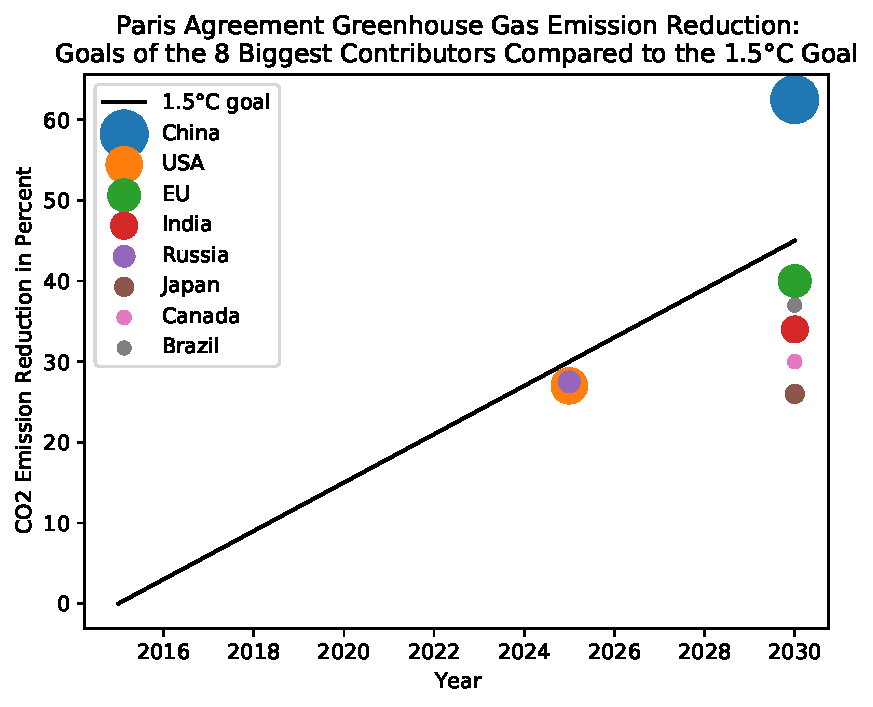
\includegraphics[width=0.5\textwidth]{img/co2goals_bubbles.pdf}}
	\caption{Goals of the 8 Biggest Contributors.}
	\label{fig:goals_lines}
\end{figure}

In conclusion, China has by far the most ambitious goals, which is even exceeding the requirements of the 1.5$^\circ C$ goal. Sadly, all of the other countries of interest are currently not even trying to achieve the 1.5$^\circ C$ goal in a treaty most countries are not even able to follow.

Comparing the emission drops from \autoref{fig:emission_drop_over_normalized_deaths} to the Paris agreement goals, one can observe an emission decrease of 20\% on average. This comes already very close to the emission drop range that is aimed for in the Paris agreement, but not quite.

The real challenge we are facing, is an emission reduction while all countries desperately try to grow their economy, mostly to the expense of mother nature.






\section{Conclusion}

From the integrated sector trends, we can see a drop in \co emissions. This can be directly attributed to the manifold effects of the pandemic. 

We tried to quantify the effect and correlate emission drops to active cases of COVID-19. On a time-series, we could not find a direct relation, especially not for all countries. We thus decided to look at the integrated emission drops and case numbers/deaths. However, one can not deduce a general trend from these two plots either. We therefore conclude that we have to discuss each country by its own.

Still, we have to answer our research question with these results. As we can see from the bubble plot of the Paris climate goals, most countries will miss the \(1.5^\circ C\) goal. We want to estimate from the plot how much the emission drop helps each country to reach its goal.

Due to the pandemic, most countries see an emission drop by over 15\% for the first half of 2020. Of course, we cannot say much about how the \co emissions will behave in the next ten years and quantifying the effect of the pandemic on countries reaching their climate goals is difficult. We want to do these calculations exemplary with Japan, as it is the country with highest gap to the \(1.5^\circ C\) goal. We see that Japan would need to further reduce its emissions by roughly 15\%. This means, that Japan needs to reduce its emissions on average by 15\% every year. We see from the total average emission drop plot that Japan reduced its emission by 22.5\% during the first half of 2020. This is just slightly more than Japan would need to reduce the emissions at least. We can do the same assessment for every country. We conclude that for every country, the emissions would need to stay permanently on a similar level as in the first half of 2020, every year, until 2030.







\section{Comments to the Group Work Experience}

\subsection*{Preferred working hours and days}

The bulk of the work was performed during the daytime. The spike at 9 am is a singularity, where one group member manually pushed 185 files because of an misunderstanding about git. Therefore, we conclude that the relevant productivity maximum was around 13 am. Afterwards, due to lunch time, the productivity decayed. Some pushes, where even performed during the night, which indicates the high commitment of the team.
\begin{figure}[h!]
\centering
\subfloat[daytime]{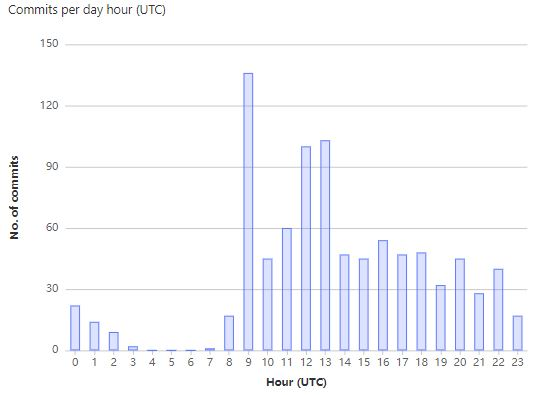
\includegraphics[width=0.5\linewidth]{group_work/hour_commits}}
\subfloat[monthday]{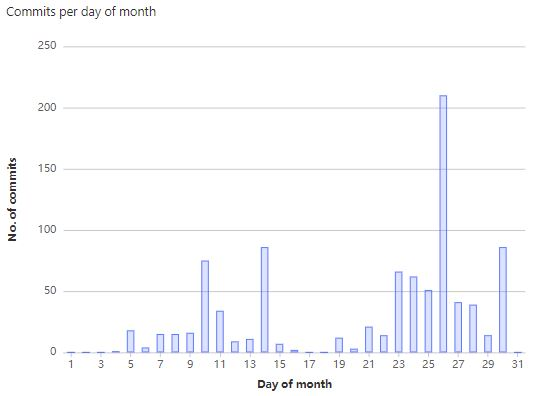
\includegraphics[width=0.5\linewidth]{group_work/monthday_commits}}\\
\subfloat[weekday]{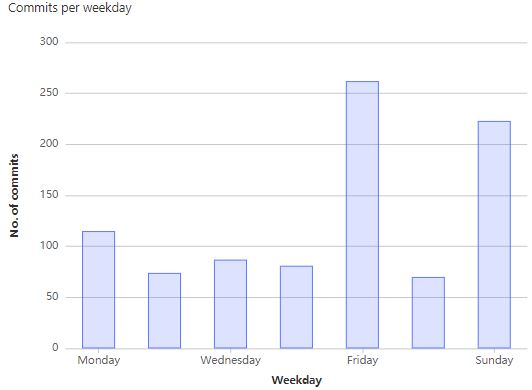
\includegraphics[width=0.5\linewidth]{group_work/weekday_commits}}
\caption{Commit histogram for different timescales.}
\label{fig:hour_commits}
\end{figure}
When we focus on a monthly scope, we can see spikes around the delivery dates at the end of the month and on the 14th for the third milestone. In a weekly scope, friday and sunday were the most populat days to push changes to the repository. This can be easily understood, when considering that the usual week of most team members was already packed with lectures, tutorials, and student jobs.

\begin{figure}[h!]
	\centering
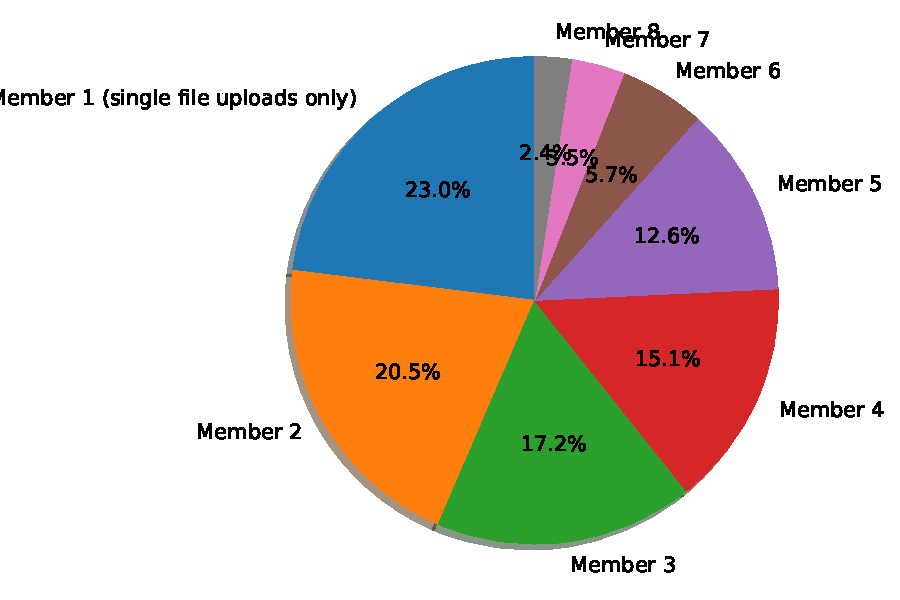
\includegraphics[width=0.7\linewidth]{group_work/name_commits}
\caption{Commits by group member.}
\end{figure}

\subsection*{Comparison to risk assessment}

Which risks where estimated wrongly?

\definecolor{lightgray}{rgb}{0.75,0.75,0.75}
\definecolor{lightergray}{rgb}{0.85,0.85,0.85}
\definecolor{slightlylightergray}{rgb}{0.92,0.92,0.92}
\def\checkmark{\tikz\fill[scale=0.4](0,.35) -- (.25,0) -- (1,.7) -- (.25,.15) -- cycle;}
\begin{center}
	\begin{footnotesize}
		\setlength{\arrayrulewidth}{1,05pt}
		\begin{tabular}[htb]{|p{2cm}|p{5cm}|p{1.5cm}|p{1cm}|p{1cm}|}
			\hline
			\textbf{Technical Risk} & \textbf{Countermeasures (CM)} &
			\textbf{Estimated prob.[\%]} &\textbf{CM needed} & \textbf{Threat avoided} \\
			\hline
			\hline
			\rowcolor{lightgray} Lack of access to data & Talk to the institution that possesses the data or ask the supervisors for access & 60.0 & \cmark & \cmark\\
			\hline	
			\rowcolor{lightgray} Lack of data & Find enough reliable resources before deciding on the final research question, & 50.0& \cmark & \cmark\\
			\hline
			\rowcolor{lightergray} Lack of knowledge & Read up things we need to learn in books or online & 40.0& \xmark & \cmark\\
			\hline
			\rowcolor{lightergray} Unreliable algorithm & Put more effort in the programming part, & 40.0&  \cmark& \cmark\\
			\rowcolor{lightergray} & Have enough team members with coding experience & &\xmark &\cmark\\
			
			\rowcolor{lightergray} & Check the references of research papers to find more data & &\cmark &\cmark\\
			\hline
			\rowcolor{lightergray} Personal biases (e.g. when categorizing data) & Try to find very objective ways to categorize data, although one can probably never be sure that this kind of bias does not occur & 40.0&\xmark & \cmark\\
			\hline	
			\rowcolor{lightergray} Bad or useless technology &  Find appropriate methods to create good model & 40.0 &\xmark & \cmark\\ 
			\hline
			\rowcolor{lightergray} Poorly formulated research question & If necessary, talk with the supervisors of the lecture whether (minor) changes are OK & 30.0 & \xmark & \cmark\\
			\hline
			\rowcolor{slightlylightergray} Data bias & try to get reliable data or at least try to find aspects which could lead to a bias in your data & 20.0& \cmark &\cmark\\
			\hline	
			\rowcolor{slightlylightergray} Insufficient idea of the project & Choose only a research question which is truly understood by the whole team & 20.0&\xmark &\cmark\\
			\hline
			\rowcolor{slightlylightergray} Irrelevant requirements & establish realistic requirements to complete the project & 10.0&\xmark &\cmark\\
			\hline	
			\rowcolor{slightlylightergray} Project too complex & With enough dedication and willpower, one can achieve everything & 10.0 &\xmark &\cmark\\
			\hline
		\end{tabular}
	\end{footnotesize}
\end{center}

\begin{center}
	\begin{footnotesize}
		\setlength{\arrayrulewidth}{1,05pt}
		\begin{tabular}[htb]{|p{2cm}|p{5cm}|p{1.5cm}|p{1cm}|p{1cm}|}
			\hline
			\textbf{Organizational Risk}& \textbf{Countermeasures (CM)} &
			\textbf{Estimated prob.[\%]} &\textbf{CM needed} & \textbf{Threat avoided} \\
			\hline
			\hline
			\rowcolor{lightgray} Poorly formulated priorities & Never formulate priorities by yourself, always work in a team! $\Rightarrow$ automatic cross-checks & 60.0&\xmark &\cmark\\
			\hline	
			\rowcolor{lightergray} Irrelevant resources & Check diligently if all resources are relevant & 40.0 &\xmark &\cmark\\
			\hline
			\rowcolor{slightlylightergray} Strong interdependence in the team & This might only be a problem in teams with poor communication and lazy students, which does not apply to our team & 10.0 &\cmark &\xmark\\
			\hline
		\end{tabular}
	\end{footnotesize}
\end{center}

\begin{center}
	\begin{footnotesize}
		\setlength{\arrayrulewidth}{1,05pt}
		\begin{tabular}[htb]{|p{2cm}|p{5cm}|p{1.5cm}|p{1cm}|p{1cm}|}
			\hline
			\textbf{Project Management Risk}& \textbf{Countermeasures (CM)} &
			\textbf{Estimated prob.[\%]} &\textbf{CM needed} & \textbf{Threat avoided} \\
			\hline
			\hline
			\rowcolor{lightgray} Wrong time estimation & This is a potentially dangerous risk, that is why time estimations have to be as precise as possible. We chose a democratic process where everybody assigns a workload he thinks is adequate to each task. The results are discussed afterwards and we decide on a time estimate together & 70.0&\xmark &\cmark\\
			\hline
			\rowcolor{lightergray} No control points & Try to set up synchronizing meetings to figure out problems with understanding or mistakes & 40.0  &\cmark &\cmark\\
			\hline
			\rowcolor{lightergray} Wrong task assignment & This is critical as well, which is why we try to let everybody assign himself to the tasks he feels comfortable with to ensure proper task assignment & 30.0 &\cmark &\cmark\\
			\hline	
			\rowcolor{lightergray} Bad team communication & Conduct weekly meetings as a minimum to synchronize the team, have more meetings if necessary & 25.0&\cmark &\cmark\\
		
			\hline
		\end{tabular}
	\end{footnotesize}
\end{center}

\begin{center}
	\begin{footnotesize}
		\setlength{\arrayrulewidth}{1,05pt}
		\begin{tabular}[htb]{|p{2cm}|p{5cm}|p{1.5cm}|p{1cm}|p{1cm}|}
			\hline
			\textbf{External Risk}& \textbf{Countermeasures (CM)} &
			\textbf{Estimated prob.[\%]} &\textbf{CM needed} & \textbf{Threat avoided} \\
			\hline
			\hline
			\rowcolor{slightlylightergray} Low working morale & Have weekly meetings as a minimum to synchronize the team, & 20.0&\cmark &\cmark\\
			\rowcolor{slightlylightergray} & have a group leader ("product owner" Philipp in our case), which is able to motivate the team & &\cmark &(\cmark)\\
			\hline
			\rowcolor{slightlylightergray} Computer crash/software error & Save all data in the cloud and have backups, & 15.0&\xmark &\cmark\\
			\rowcolor{slightlylightergray} & ask the university for rental laptops if a computer stops working completely & &\xmark &\cmark\\
			\hline	
			\rowcolor{slightlylightergray} Changes by supervisors of the lecture & We estimate the probability of this to happen as very low but we are sure that we could talk to the supervisors if problems arise from such changes & 5.0&\xmark &\cmark\\
			\hline
		\end{tabular}
	\end{footnotesize}
\end{center}
	%todo: spell check
	In summary, all technical risks could be avoided. The most important countermeasures where taken against the lack of data: We continously searched for more datasets when we changed our approach. 
	
	
	
	Organizational risks posed a challenge in an unexpected threat. Sometimes, team members could only be motivated by very short deadlines, which impeded the report writing. 
	
	%todo: formulate nicer
	We as a team always came up with a solution to tackle the problem and managed to deliver every milestone on time and with a good quality. The team had exceptional communication and team skills and responsibly shifted tasks when team members had time limitations or a weak internet connection.
	
	\section*{Updated time schedule}
	
	After 16 weeks of team work including multiple project deadline extensions, we want to give an update of the initial time schedule we handed in together with the research proposal. At a first glance, the changes in the deadlines of the milestones can be observed. Also, one will notice that the buffers shrinked to mostly one day. Initially, we planned approximately one week buffer for each milestone. This can be interpreted as that the buffers were calculated completely right, since there was always at least one day buffer remaining in the end and we were able to finish the project milestones in time. Still, the buffers shrinked due to problems which occured as we were working on the milestones. This behavior was to be expected and that is the reason why we included buffers. 
	
	Another major change was the front end task schedule. In contrast to the initial plan, we already started working on the front end in the second milestone in order to have an interactive visualization of the datasets we collected. This front end was kept up-to-date and extended during the rest of the project.
	
	Especially for milestone three, the task durations could be increased significantly due to the deadline extension until the 14th of August which was related to the exam period we went through. For all the other milestones, various minor changes in task durations and task schedules can be seen.
	
	The updated time schedule is shown in the following Figure \ref{fig:updated_time_schedule}.
	
	\begin{figure}[H]
		\centering
		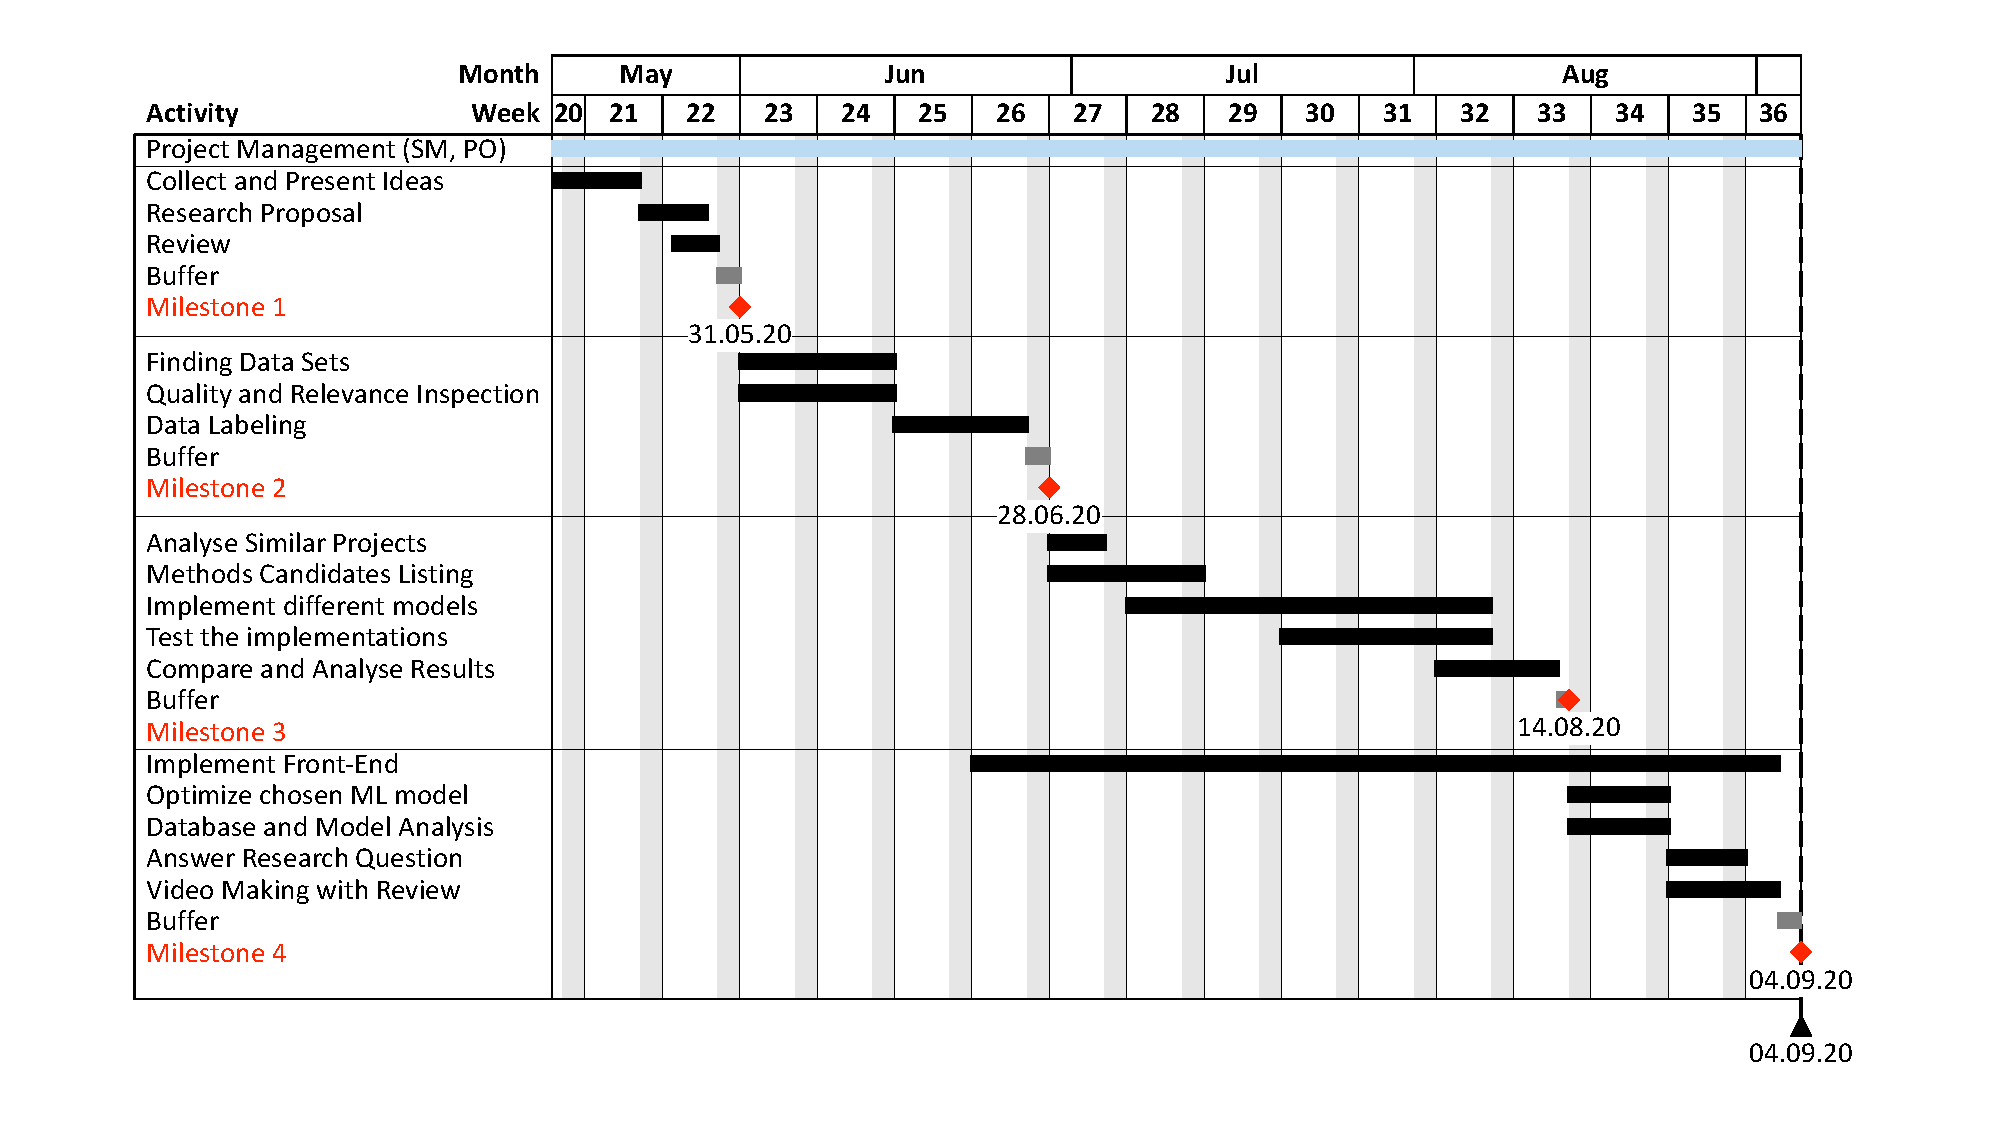
\includegraphics[width=\textwidth]{img/updated_time_schedule}
		\caption{Updated Time Schedule.}
		\label{fig:updated_time_schedule}
	\end{figure}
	
	

\include{update_timeline}

\bibliographystyle{unsrt}
\bibliography{references}


\end{document}
